\documentclass[12pt,a4paper]{report}

\makeatletter

\def\author#1{\gdef\insertauthor{#1}\gdef\@author{#1}\hypersetup{pdfauthor={#1}}}
\def\title#1{\gdef\inserttitle{#1}\gdef\@title{#1}\hypersetup{pdftitle={#1}}}
\def\keywords#1{\gdef\insertkeywords{#1}\hypersetup{pdfkeywords={#1}}}
\def\subject#1{\gdef\insertsubject{#1}\hypersetup{pdfsubject={#1}}}

\makeatother

\RequirePackage[final,breaklinks,bookmarks]{hyperref}

\hypersetup{%
    colorlinks=true,
    allcolors=blue,
    pdfcreator  = {\LaTeX\ with package \flqq hyperref\frqq},
    pdfproducer = {pdfeTeX-0.\the\pdftexversion\pdftexrevision}
}


%############################################################################
%########################### Change This ####################################
%############################################################################
%replace with German "Bachelor Thesis", "Master Thesis" or "Diplomarbeit" or
%replace with English "Bachelor's Thesis", "Master's Thesis"  
\subject{Bachelor's Thesis}
%put your title here
\title{Assessing Camera Placement Proposals for Autonomous Driving Infrastructure}
%your name
\author{Georgi Kotsev}
%your matrikelnummer
\newcommand{\trmatrikelnummer}{410112}
%supervisor
\newcommand{\trbetreuerA}{Dipl.-Inf. Martin Berger}
%reviewer one
\newcommand{\trguta}{Prof. Dr. Dr. h.c. Sahin Albayrak}
%reviewer two
\newcommand{\trgutb}{Prof. Dr. Odej Kao}
\date{\today}
%put some meaningful keywords, these are only examples
\keywords{Multi-Agent Systems, Machine Learning}

%###################################################################################
%###################### Document Defintions ########################################
%###################################################################################
%aubrey: no real need to change these
%how to handle spaces
\sloppy
\makeindex

\usepackage[utf8]{inputenc}
\usepackage{amsmath, marvosym} % Mathematik
%\usepackage{harvard} %for harvard style citation, keep this position before url package
\usepackage{times, url, geometry, amssymb, booktabs}


%\usepackage[pdfusetitle]{hyperref}
\usepackage[pdftex]{graphicx} %pdf figures
%\usepackage[pdftex,
%            pdfauthor={Your Name},
%            pdftitle={The Title},
%            pdfsubject={The Subject},
%            pdfkeywords={Some Keywords},
%            pdfproducer={Latex with hyperref, or other system},
%            pdfcreator={pdflatex, or other tool}]{hyperref}
\usepackage{subfig} %multi-figures
\usepackage{listings} %code listings
\usepackage{multirow} %for multi-row tables
\usepackage{color} %needed for listings
\usepackage{svg}
\usepackage{subfig}
\usepackage{xcolor}
\newcommand\myworries[1]{\textcolor{red}{#1}}


%depth of section
\setcounter{secnumdepth}{4}
%depth of TOC
\setcounter{tocdepth}{3}
%directory for graphics
\graphicspath{{gfx/}}

%setting for listing
\lstset{
	extendedchars=true,
	basicstyle=\scriptsize\ttfamily,
	%basicstyle=\tiny\ttfamily,
	tabsize=2,
	keywordstyle=\textbf,
	commentstyle=\color{grau},
	stringstyle=\textit,
	numbers=left,
	numberstyle=\tiny,
	% für schönen Zeilenumbruch
	breakautoindent  = true,
	breakindent      = 2em,
	breaklines       = true,
	postbreak        = ,
	%prebreak         = \raisebox{-.8ex}[0ex][0ex]{\ensuremath{\lrcorner}},
	prebreak         = \raisebox{-.8ex}[0ex][0ex]{\Righttorque},
}

%Table of Content TOC settings
\setcounter{tocdepth}{3}
%This is needed for entering URLs for harvard citation style
%\renewcommand{\harvardurl}{URL: \url}


%###################################################################################
%########################### Thesis content ########################################
%###################################################################################
\begin{document}
%__________________________Start_of_Thesis______________________________________________
%Roman numeral numbering for initial section of thesis
\pagenumbering{roman}
%title page specification, deployed as seperate file the input folder

%############################################################################
%########################### DO NOT touch this, unless you need to ##########
%############################################################################
\makeatletter
\thispagestyle{empty}
%head line logo + tub + logo
\begin{tabular}{lcc}
\includegraphics[width=0.15\textwidth]{template/TUBerlin_Logo_rot_hell}& \hspace{1.1cm} Technische Universit{\"a}t Berlin& \hspace{1.2cm} 
\includegraphics[width=0.15\textwidth]{template/aot_logo}\\
\end{tabular}
%draw a line
\rule{\textwidth}{0.4pt}
%aub: remove this on final submission
\begin{center}
DOCUMENT BUILD DATE: \today\\%
%add your status here, e.g. First Draft for Supervizor etc.
DOCUMENT STATUS: Beta
\end{center}

%vertical space
\vspace{2.5cm}
\begin{center}
%replace this
  \textbf{\LARGE \@title}
\end{center}
\vspace{2cm}

\begin{center}
  \textbf{\insertsubject} \\
  am Fachgebiet Agententechnologien in betrieblichen Anwendungen und der Telekommunikation (AOT)\\
  Prof.\ Dr.-Ing.\ habil.\ Sahin Albayrak \\
  Fakultät IV Elektrotechnik und Informatik \\
  Technische Universität Berlin \\[0.5cm]
  vorgelegt von \\
  \textbf{\@author}
\end{center}

\vspace{1cm}


\begin{center}
\begin{tabular}{ll}
Betreuer: & \trbetreuerA, \\ 
Gutachter:& \trguta\\
& \trgutb\\
\end{tabular}
\end{center}

\vfill

\begin{tabular}{l}
\@author \\
Matrikelnummer:  \trmatrikelnummer \\
\end{tabular}

\rule{\textwidth}{0.4pt}
\makeatother
\clearpage

%abstract plus acknowledgement and statement
%#############################################################
%###################### Statement ############################
%#############################################################
\chapter*{Erkl{\"a}rung der Urheberschaft}
%this one needs to be signed for submission
Ich erkläre hiermit an Eides statt, dass ich die vorliegende Arbeit ohne Hilfe Dritter und ohne Benutzung anderer als der angegebenen Hilfsmittel angefertigt habe; die aus fremden Quellen direkt oder indirekt übernommenen Gedanken sind als solche kenntlich gemacht. Die Arbeit wurde bisher in gleicher oder ähnlicher Form in keiner anderen Prüfungsbehörde vorgelegt und auch noch nicht veröffentlicht.


\vspace{4cm}

Ort, Datum:\hspace{0.25cm} Berlin, den 21.12.2022 \hfill Unterschrift: \hspace{1cm}

%#############################################################
%###################### Abstract  ############################
%#############################################################
\newpage
\chapter*{Abstract}
% DELETEME: An abstract is a teaser for your work. You try to convince a reader that it is worth reading your work. Normally, it makes sense to structure you abstract in this way: 
% \begin{itemize}
% \item one paragraph on the motivation to your topic
% \item one paragraph on what approach you have chosen
% \item and one paragraph on your results which may be presented in comparison to other approaches that try to solve the same or a similar problem.
% \end{itemize}
% Abstract should not exceed one page (aubrey's opinion)

%#############################################################
%###################### German Abstract ######################
%#############################################################
\newpage
\chapter*{Zusammenfassung}
% DELETEME: translate to German to English or vice-versa.

%#############################################################
%###################### Acknowledgements #####################
%#############################################################
\newpage
\chapter*{Acknowledgements}
For the constant support during the implementation of the code and the writing whenever problems occured I want to thank Martin Berger. Hereby I thank the authors of this template, for the endless efforts to help me and enhance my work.

%TOC
\tableofcontents
%add list of figures to TOC
\cleardoublepage
\addcontentsline{toc}{chapter}{List of Figures}
\newpage
\listoffigures
%add list of tables to TOC
\cleardoublepage
\addcontentsline{toc}{chapter}{List of Tables}
\newpage
\listoftables

%__________________________Main_Content______________________________________________
\newpage
%from now on, numbering should be arabic
\pagenumbering{arabic}
\chapter{Introduction}
%labels will help you to reference to certain images, tables, chapters, section, and so on...
\label{introduction}
This chapter presents an explanation about what has served as motivation for this thesis. What else is provided are the approach for solving the issue as well as the aims of the work. At the end of the chapter, the structure is defined.

%###################################################################################
%###################### Motivation          ########################################
%###################################################################################
\section{Motivation}
In recent times, the amount of interest in a cooperative environment for autonomous vehicles and infrastructure has increased and there are many researches on this topic \cite{ cvis_article_one, cvis_article_two}. Its main goal is to increase safety, decrease number of accidents and improve efficiency of city traffic. In order to achieve this it must be guaranteed that the self-steering vehicles are aware of their surroundings during the whole ride \cite{onboard_sensors}.

Nowadays, the cars with the highest level of autonomy\footnote{\url{https://www.auto123.com/en/news/vehicle-autonomy-levels-explained/64372}, visited on 13/11/2022} integrate a combination of sensors like radar, Light Detection and Ranging (LiDAR) and camera systems to be able to perceive other traffic participants \cite{autonomous_cars_sensors}. In spite of their widespread adoption in the automobile industry for guaranteeing a high level of safety and driving facilitation, on-board sensors have their drawbacks like limited visibility and decreased field of perception. Another issue is that vehicle-integrated sensors cannot have a clear estimation when there is an object that impedes their field of view (FoV). Thus, the use of stationary sensors in a city infrastructure is beneficial for providing more reliable and accurate information \cite{roadside_lidar}. Moreover, placement of sensors in the road area expands significantly the vehicle's range of view and contributes to safer and congestion-free roads. Unlike other sensors, cameras are cheaper and much easier to maintain\footnote{\url{https://www.autopilotreview.com/lidar-vs-cameras-self-driving-cars/}, visited on 13/11/2022}. Another advantage is that they are capable of seeing the world like a human being would do, which is of utmost importance in object detection and tracking algorithms \cite{camera_object_detection}. The highly researched camera technology and its features are main reasons for this thesis to focus on its usage for aiding autonomous driving.

Real-world experiments for investigating which sensor placement is optimal should always be planned precisely and require careful preparation because of various factors that can impact the results. In addition, conducting tests in the real world results in more costs and effort to reproduce a specific scenario. For the purpose of reducing costs and considering a greater range of camera positioning options, this work relies on the 3D autonomous driving simulator Carla\footnote{\url{https://carla.org/}, visited on 13/11/2022}. It is used for generating simulated data samples for different camera placements, which is then evaluated by using heatmaps and the results are summarized.

DELETEME: Example for a chain: Mobile communication gets increasingly popular in the world (CITE sales on mobile communication infrastructure, mobile phones, or increasing number of mobile phones contracts). $\rightarrow$ Especially smartphones, which represent the next generation cellular phone (CITE), get more and more used for communicating not only with other people but also for connecting to the Internet for using various services (CITE). $\rightarrow$ Smartphone are comprehensive cellular phones that provide additional functionality due to their increased connection and processing capabilities (CITE). $\rightarrow$ Most smartphones offer an online application store for adding software to the devices which helps the users to customize their devices according to their needs, e.g. Android Market\footnote{\url{http://market.android.com}, visited on 05/08/2011}. $\rightarrow$ One problem about installing third-party software is that not all software try to help the user; $\rightarrow$ software with malicious intentions, so-called malicious software (malware), can be a severe threat to smartphone users. Some malware delete files (EXAMPLE + CITE or footnote with URL) or even destroy devices (EXAMPLE + CITE or footnote with URL). $\rightarrow$ More and more smartphone malware appeared in the last years (CITE). $\rightarrow$ Signature-based approaches work efficiently on known malware (CITE) but face serious drawbacks regarding unknown malware. $\rightarrow$ Oberheide et al.~\cite{oberheide:2008:cloudav} state that virus engines need an average time of 48 days until their databases get updated to be able to detect a certain unknown malware. $\rightarrow$ This in turn means that smartphone users stay unprotected for this time, which can be seen as a severe threat. $\rightarrow$ Therefore, approaches are needed that are capable of detecting unknown malware for protecting the users against such threats.
DELETEME: This example showed how one could argue that alternative approaches for malware detection is required. The length of the motivation depends on the topics handled and can of course be longer. The principle I am describing is also shown on Figure~\ref{fig:writing}

\begin{figure}
\centering
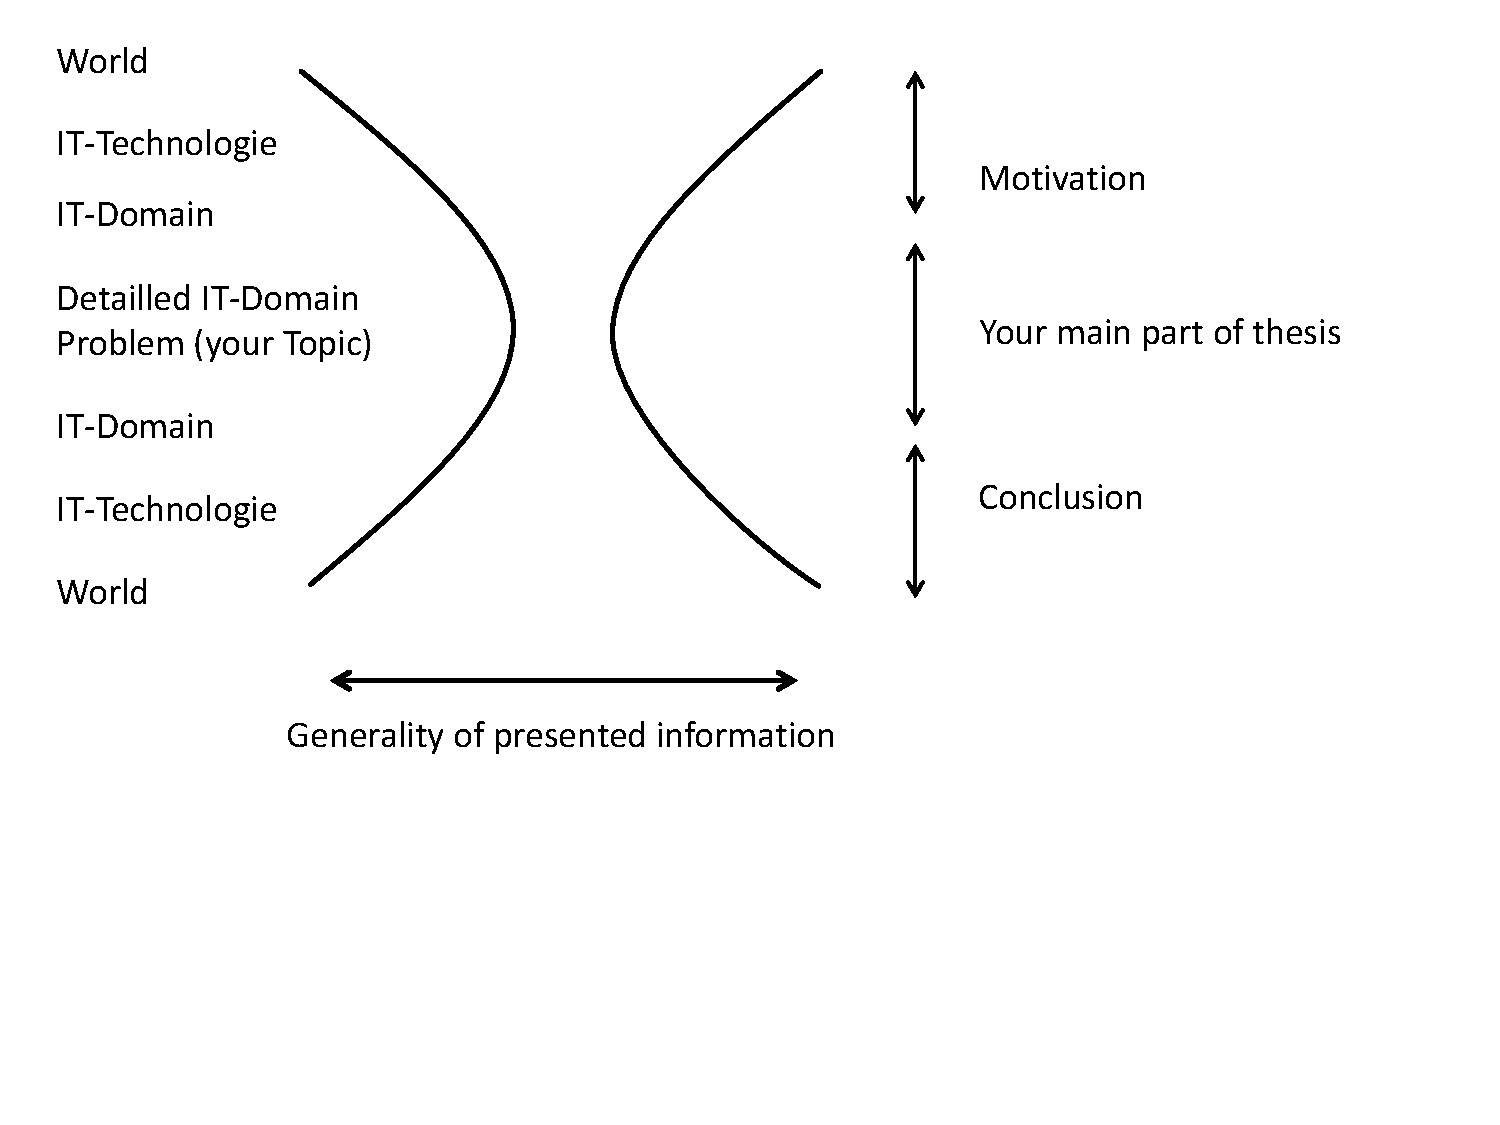
\includegraphics[width=0.9\textwidth]{template/writing}
\caption[Information Generality]{This images illustrates how generality of information could be handled in a thesis. In your motivation you should start from a very broad view on the topic. Then you should get more precise with every statement until you reach the actual problem you are addressing. You should do vice-versa in your conclusion, starting with the problem that you addressed and getting broader until you can write about the meaning of your results to the (IT-)world.\label{fig:writing}}
\end{figure}


%###################################################################################
%###################### Approach and Goals  ########################################
%###################################################################################
\section{Approach and Goals}
DELETEME: In this section, you should cleary describe your approach that you are following in order to solve the underlaying problem of your thesis. Additionally, you should clearly state the goals of your work. This will not only help you supervizor to understand what you are doing, it will also help you to be sure on which topic you should evaluate.

The main goal of this thesis is to estimate an optimal camera position and its configuration using a simulated environment, where no real-world limitations occur. For the approach all simulations are executed on a junction of four roads as it is considered being the one with most conflict points by the European Road Safety Observatory\footnote{\url{https://www.dacota-project.eu/Links/erso/knowledge/Content/15_road/junctions.html}, visited on 13/11/2022}. We place a stationary monocular camera in the infrastructure in such positions that a greater range of interest (ROI) lands in the sensor's FoV. During the experiments, we spawn two static vehicles on all possible points, which the junction contains and which are captured on the image plane. As a following step, we apply a mathematical model - Occlusion Degree Model (ODM) \cite{occlusion_degree_model} - for estimation of the percentage, which expresses the part of the target vehicle that is occluded by the occluder vehicle. With the help of the model and an instance segmentation camera \cite{instance_segmenatation_cam}, this work estimates the efficiency of different camera placement options. On every captured image the pixels containing vehicles are coloured based on their ID in the Unity Engline\footnote{\url{https://www.unrealengine.com/de/blog/welcome-to-unreal-engine-4}, visited on 14/11/2022}. Having this data, we extract the covered area of the target vehicle after each spawn and summarize the results in a heatmap. Finally, we compare the results and select the ones, which perceived as less occlusion as possible in various vehicle placement combinations. 


%###################################################################################
%###################### Structure of the Thesis ####################################
%###################################################################################
\section{Structure of the Thesis}
DELETEME: This section does not require eloquent writing. It is just a presentation of what you will handle in each chapter starting with Chapter~\ref{background}.

DELETEME: Example: This thesis is structured as follows. In Chapter~\ref{background}, we discuss essential background related to the thesis topic. (SOME MORE SENTENCES). Chapter~\ref{mainone} represents a detailed analysis of the problem that will be addressed. In particular, (SOME MORE SENTENCES). In Chapter~\ref{maintwo}, our solution is presented. This solution covers ... (SOME MORE SENTENCES). Chapter~\ref{evaluation} evaluates our solution basing on our specified goals. (SOME MORE SENTENCES). In Chapter~\ref{conclusion}, we conclude. Chapter~\ref{appendices} gives additional related information on the topic of this thesis.

The next chapters of this thesis are structured as follows: 
\begin{itemize}
    \item Chapter 2 talks about scientific information regarding camera, etc.
    \item Chapter 3 reveals some state-of-the-art methods for sensor placement, etc.
    \item In chapter 4 the problem that this thesis is concerned with and an approach for solving it are presented.
    \item Chapter 5 introduces the results of the conducted experiments and delivers insight into how they were evaluated.
    \item In the 6. Chapter we summarize the outcome of our experiments and discuss the possible tasks for a future work on this issue.
\end{itemize} 

\chapter{Scientific Background}
%labels will help you to reference to certain images, tables, chapters, section, and so on...
\label{background}

% DELETEME: This chapter will cover all of your background information and related work. Background and related work are directly related to your thesis. Please do not place irrelevant content here which is a common mistake. Citing will be handled in the appendices.

% DELETEME: Background represents underlying knowledge that is required to understand your work. The expected knowledge level of your readers can be set to the one of a bachelor or master student who just finished his studies (depending on what kind of thesis you are writing). This means that you do not need to describe how computers work, unless your thesis topic is about this. Everything that an average alumnus from your field of studies should know does not need to be described. It turns, background information that is very complex and content-wise very near to your problem, can be placed in the main parts. Everything else should be written here. Note: it is important to connect each presented topic to your thesis. E.g. if you present the ISO/OSI layer model you should also write that this is needed to understand the protocols you plan to develop in the main parts.

% DELETEME: Related work represents results from work that handled the same or a similar problem that you are addressing. This work might have used a different approach or might not have been that successful. Finding a paper / work that solved your problem in the same way you were planning to do is not good and you should contact your supervisor for solving this issue. Again, each paper / work has to be connected to your approach: other papers might have not chosen an optimal solution; they might not have been taking care of essential aspects; they might have chosen a different approach and you believe, yours will work better ...

This chapter introduces some important scientific fundamentals for better understanding of the problem's solution. Initially, \ref{camera_section} explains about the composition of a single digital pinhole camera and some of its characteristics. Then, \ref{camera_model} outlines the mathematical model for transforming a 3D object on the 2D image plane, after which the subsection \ref{instance_camera} informs about the functionality of the instance segmentation camera that CARLA offers. Finally, section \ref{carla_background} describes how the 3D autonomous driving simulator works and presents some of its features used in this work.

%###################################################################################
%###################### Topic A             ########################################
%###################################################################################
\section{Camera}\label{camera_section}
The digital camera is an instrument used for creating images through light capturing. On the figure \ref{fig:camera_construction} we could get an idea of how this technological invention is constructed. It uses an optic that consists of one or more lenses, through which the light rays are received. Afterwards, there is a sensor resembling the form of a solar panel, divided into red, green and blue pixels, which is hit by the collected light rays. As described from Schreer in \cite{camera_pinhole_model} the process of transforming the information from the captured light into a meaningful for the human eye representation is the following one: 
\begin{itemize}
    \item Light ray hits a sensor's pixel $\rightarrow$ The sensor converts it into an energy signal, which sends to the built-in computer $\rightarrow$ The computer estimates how dark or light the according pixel on the image plane should be and determines the correct colour value $\rightarrow$ As an output all pixels are combined in order to approximately recreate all details from the captured object  
\end{itemize}

\begin{figure}[h]
\centering
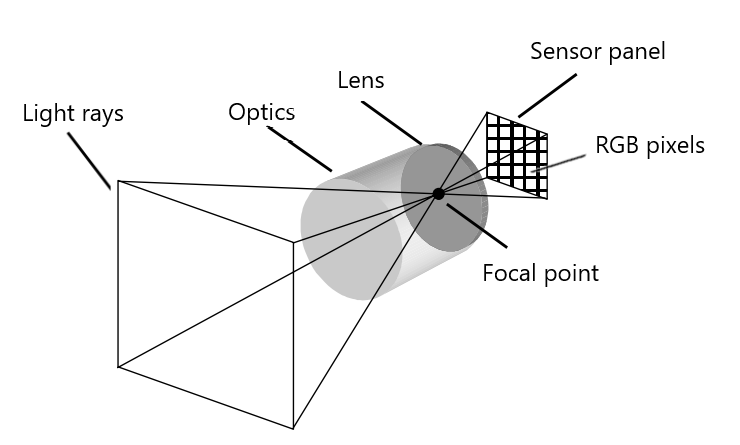
\includegraphics[width=0.8\textwidth]{images/camera_construction.png}
\caption[Digital camera's design]{This image illustrates simply the design of a digital camera, based on Schreer's book \cite{camera_pinhole_model} \label{fig:camera_construction}}
\end{figure}

\newpage
In order to display a more detailed version of the captured image, cameras need more pixels to collect light rays\footnote{\url{https://www.creativelive.com/photography-guides/how-does-a-camera-work}, visited on 18/11/2022}. Thus, modern cameras rely on a bigger number of pixels to enhance the quality of the photos, which also contributes to improving the resolution of the visual sensor. Cameras with greater resolution are important in the area of street surveillance because in case of accidents or an against-the-rules behaviour it facilitates the task of recognising the suspect. Moreover, when we take into account the fact that these sensors act as a visual world perception for the autonomous vehicles, the resolution plays an essential role in the efficient object detection \cite{resolution_importance}. 

Another specification of cameras that this thesis considers is the so-called field of view (FoV), which determines the quantity of information that has been captured on the result image. It depends on the focal length of the lens and the sensor's size. On figure \ref{fig:camera_fov} is shown what happens when the light goes through the lenses. In the upper case, due to a shorter focal length\footnote{The length between the lens and the focused image on the sensor} the lens converges the light stronger, therefore the focus is on the subject being imaged and the FoV is larger. In the vice-versa situation, the longer focal length allows for a focus on the image and thus provides a smaller FoV.

The monocular cameras belong to the directional sensors, because they can perceive information only from the direction in which their optical part is adjusted. In contrast to LiDAR sensors, which has a 360$^{\circ}$ view of the environment around it and can not be affected by light
conditions, single cameras are unreliable when exposed to bad light and weather conditions \cite{camera_vs_lidar}. As a main drawback of single cameras is regarded the lack of depth information, which impedes an accurate object recognition. Nevertheless, monocular cameras have advantages like lower integration price, much bigger availability on the market and the most important one is that they provide detailed pixel intensity information in form of a visual representation of the real world.

\begin{figure}[h]
\centering
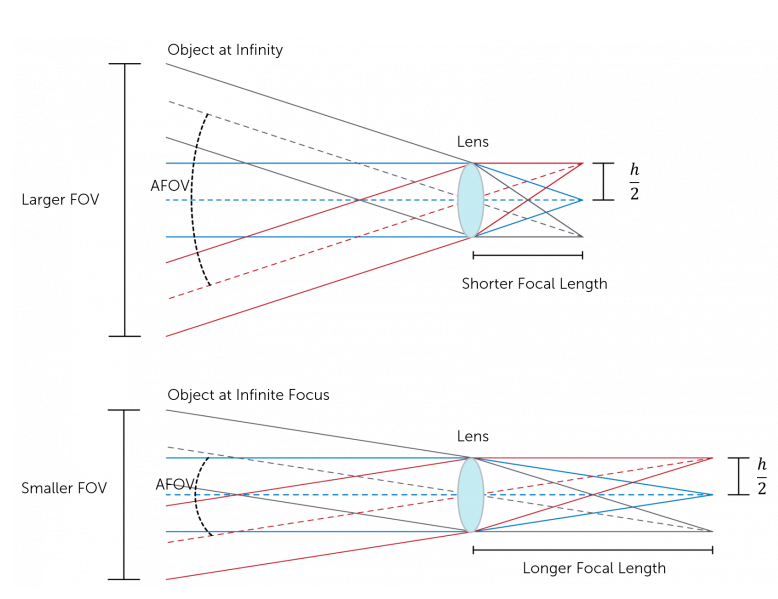
\includegraphics[width=0.8\textwidth]{images/camera_fov.png}
\caption[Single camera's FoV]{Depicting the influence of the focal length on the field of view, authored by \cite{camera_fov_website} \label{fig:camera_fov}}
\end{figure}

\subsection{Camera model}\label{camera_model}
In order to illustrate how the transformation from a 3D world coordinate point to a 2D sensor's coordinate system happens, we use the pinhole camera model from Schreer \cite{camera_pinhole_model}. Figure \ref{fig:camera_model} portrays how a point $M(X_{w}, Y_{w}, Z_{w})$ from a real world's object placed in front of the camera is orthogonally projected on the image plane. We then get the point $m$ defined in the image plane's coordinate system as $(u,v)^{T}$. As we can see, the projection center stays behind the image plane and its optical axis points in the Z-direction, therefore it intersects the image plane in the centre point $c$. When we want to define the location of a 3D world point on the image plane we have to use the camera's intrinsic matrix $A$, which contains parameter of the camera like the coordinates of the centre point $c(u_{0},v_{0})$ and the distance $\alpha = focal \: length / pixel \: size$, measured in pixels units. In the following equation we execute a matrix multiplication between the intrinsic matrix $A$ and a normalized 3x4 matrix $P_{N}$:

\begin{equation}
    P_{new} = A P_{N} = \begin{bmatrix}
                        \alpha & 0 & u_{0}\\
                        0 & \alpha & v_{0}\\
                        0 & 0 & 1\end{bmatrix} \cdot \begin{bmatrix}
                        1 & 0 & 0 & 0\\
                        0 & 1 & 0 & 0\\
                        0 & 0 & 1 & 0\end{bmatrix}
\end{equation}

As an output of the equation we receive the projection matrix $P_{new}$ and the last step is to transform the world coordinates of the point $M$ into the sensor's coordinate system. This is done by applying another multiplication between a Euclidean homography matrix $H$ and the point $M$ coordinates, after which we finally multiply the projection matrix with the result. The above-mentioned process is the following one:

\begin{equation}
m = P_{new} \cdot H \cdot M
\end{equation}

\begin{figure} [h]
\centering
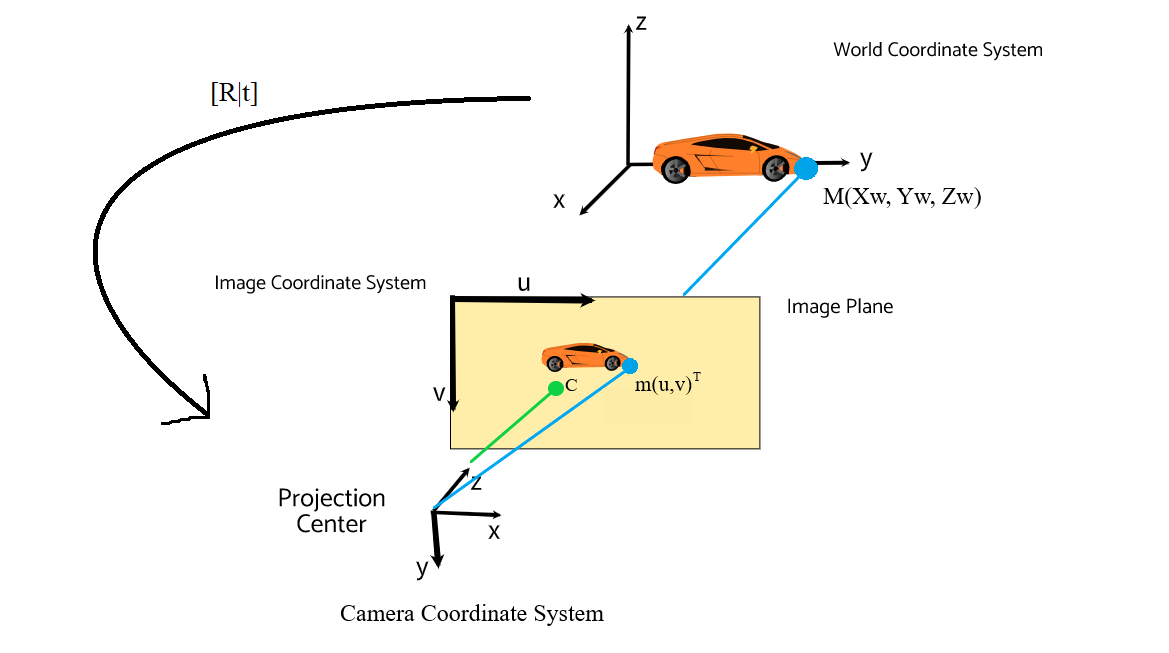
\includegraphics[width = \textwidth, height = 10cm]{images/camera_model_pic.png}
\caption[Single camera's model]{Scheme of the pinhole model and a projection of a 3D object on a 2D image plane, based on \cite{camera_pinhole_model} \label{fig:camera_model}}
\end{figure}

%###################################################################################
%###################### Topic B             ########################################
%###################################################################################
\section{CARLA - 3D autonomous driving simulator}\label{carla_background}
In this section we introduce the open-source 3D simulator CARLA (Car Learning to Act) which runs as a layer over Unreal Engine 4 with the main purpose of facilitating autonomous driving research. The simulation platform provides a great number of open digital assets like buildings, vehicles, pedestrians, whole cities, etc. What is more, the simulator is constantly developed by a community of different developers, who contribute to a realistic digital environment and an efficient conducting of experiments and tests. In addition to the aforementioned benefits, CARLA gives the opportunity to researchers to work with urban layouts without having to consider any logistical difficulties of training and testing systems in the physical world or infrastructure costs \cite{carla_paper}. 

In contrast to the real world, inside the Unreal-Engine based platform users are not limited to using a couple of vehicles, which enables them to cover a multitude of edge cases that are necessary for training and validation. Experiments often involve some kind of sensor, whose implementation and setup could be expensive and time-consuming, thus we use CARLA for this work, because it offers various types of sensors\footnote{\url{https://carla.readthedocs.io/en/latest/ref_sensors/}, visited on 20/11/2022} like RGB camera, depth camera, instance and semantic segmentation camera, LiDAR and radar systems.

CARLA is developed as a client-server application, where the client communicates with the server through sockets. The client API is programmed in Python, and realises an interaction with the server by sending user-implemented Python scripts in return for sensor data. Simultaneously, the server's task is to render the received client data in a running simulation. There are two types of commands that the client could send:
\begin{itemize}
    \item \textbf{normal commands} - control the world actors like vehicles or pedestrians and can modify all their attributes
    \item \textbf{meta-commands} - reset the simulation, define the server's behaviour, are responsible for the sensors and can apply different environmental settings like weather conditions or traffic density
\end{itemize}

Figure \ref{fig:carla_arch} presents a more detailed view about the scalable client-server architecture CARLA runs on. The server uses Unreal Engine 4 and Carla Plugins to create a realistic simulation of an urban environment, whereas the client communicates with it over TCP. This type of architecture allows multiple clients to connect with the server at the same time, although it is advisable to avoid it, because these are controlled by the developer and collisions could appear. It can be seen on the diagram that the CARLA API combines Python scripts and C++, which bring with itself the benefits of an uncomplicated environment for developers and a lower-lever robust communication. When the client is already connected to the server it can control the world actors and their behaviour as well. For instance, it uses a traffic manager to recreate a real-life traffic situations and define speed, direction, acceleration or other vehicle's attributes.

\begin{figure} [h]
\centering
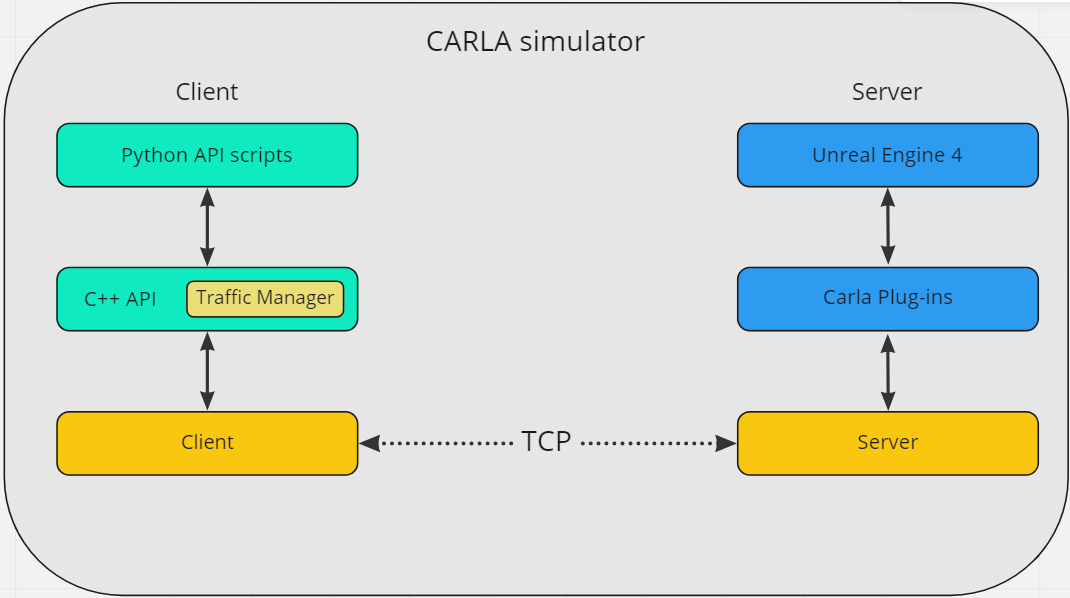
\includegraphics[width = 0.9\textwidth]{images/carla_arch.png}
\caption[CARLA's architecture]{Scheme of CARLA's client-server architecture, based on \cite{carla_architecture} \label{fig:carla_arch}}
\end{figure}

\subsection{RGB and Instance Segmentation Camera}\label{instance_camera}
In the above section we mentioned that CARLA supports different sensor types, among which the RGB and instance segmentation camera, which are the main focus of this thesis. The user defines a location in the simulator's world coordinates where a sensor should be spawn and apart from that the rotation of the sensor is adjusted to retrieve data from a specified direction. Furthermore, CARLA provides various basic and advanced camera attributes like FoV, image width, image height, lens distortion, calibration constant, etc\footnote{\url{https://carla.readthedocs.io/en/latest/ref_sensors/\#rgb-camera}, visited on 20/11/2022}. The output of the RGB camera is sensor-related information and raw data, which contains an array consisting of BGRA (blue, red, green and opacity index) 32-bit pixels.

For the purpose of a better differentiation between objects of the same type, CARLA implements the instance segmentation camera\footnote{\url{https://carla.readthedocs.io/en/latest/ref_sensors/\#instance-segmentation-camera}, visited on 20/11/2022}. Unlike the RGB camera, this one does not display the object's real colours. It classifies them by class and instance ID, during which a tag is assigned to every pixel on the image plane according to the type of object (vehicle, building, road, traffic sign, etc) it contains \cite{instance_segmenatation_cam}. In the output we receive again a BGRA array, but the pixels consist of the following colour values:
\begin{itemize}
    \item \textbf{Red channel} - contains a tag value from 0-22, for each type of object it belongs to. Apart from the pre-defined tags, the user can create new ones.
    \item \textbf{Green and Blue channel} - provide information about the internal ID of the object, which was set when it was initialised from Unreal Engine. We can retrieve the ID by solving this equation: $ID \: =  B + G * 256$
\end{itemize}

The information we get from an instance segmentation camera is useful for experiments, where we lack depth data and do not know whether one vehicle is located in front of another one. Moreover, the ground truth data contributes to more accurate and reliable results from the conducted experiments. To get an idea of the colour palette that the two cameras apply, we can have a look at the pictures below in Figure \ref{fig:camera_outputs}. 

\begin{figure} [h]
  \centering
  \subfloat[RGB camera]{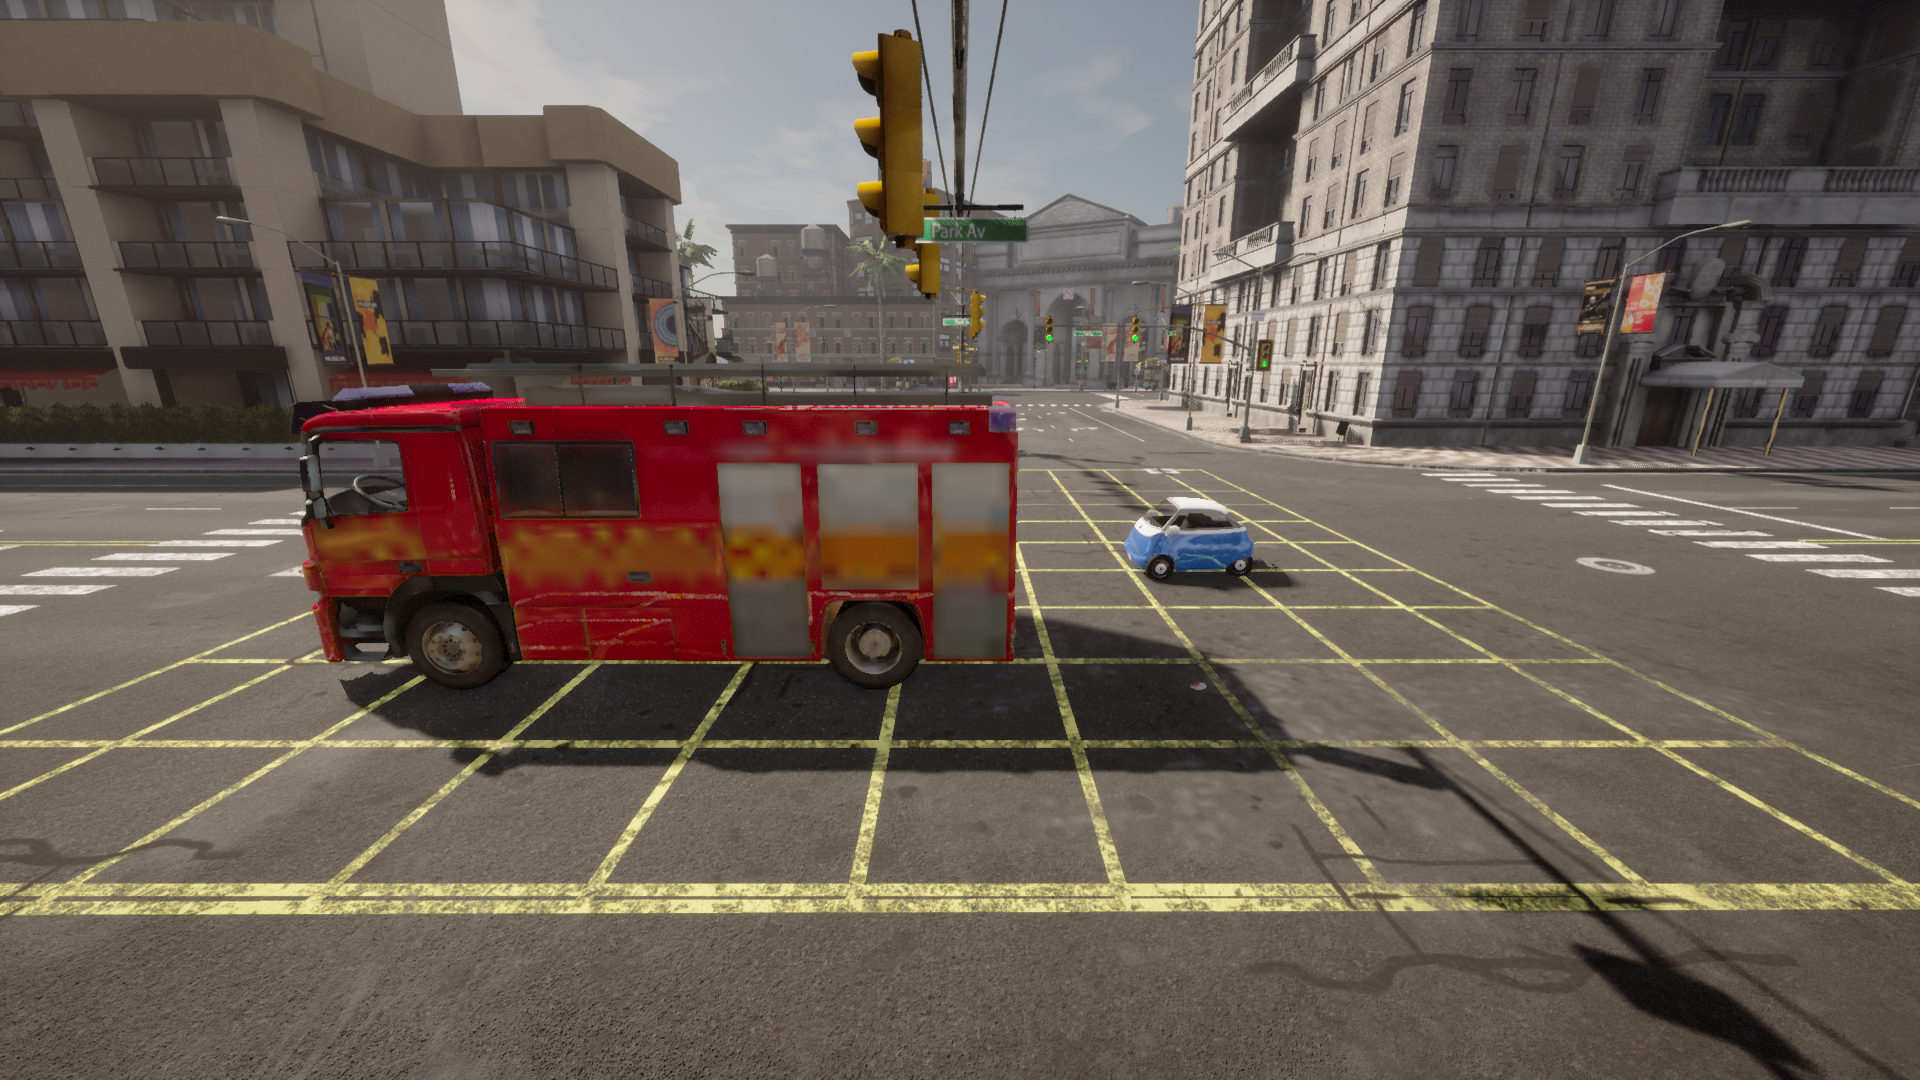
\includegraphics[width=0.5\textwidth]{images/rgb_cam.jpg}}
  \hfill
  \subfloat[Instance segmentation camera]{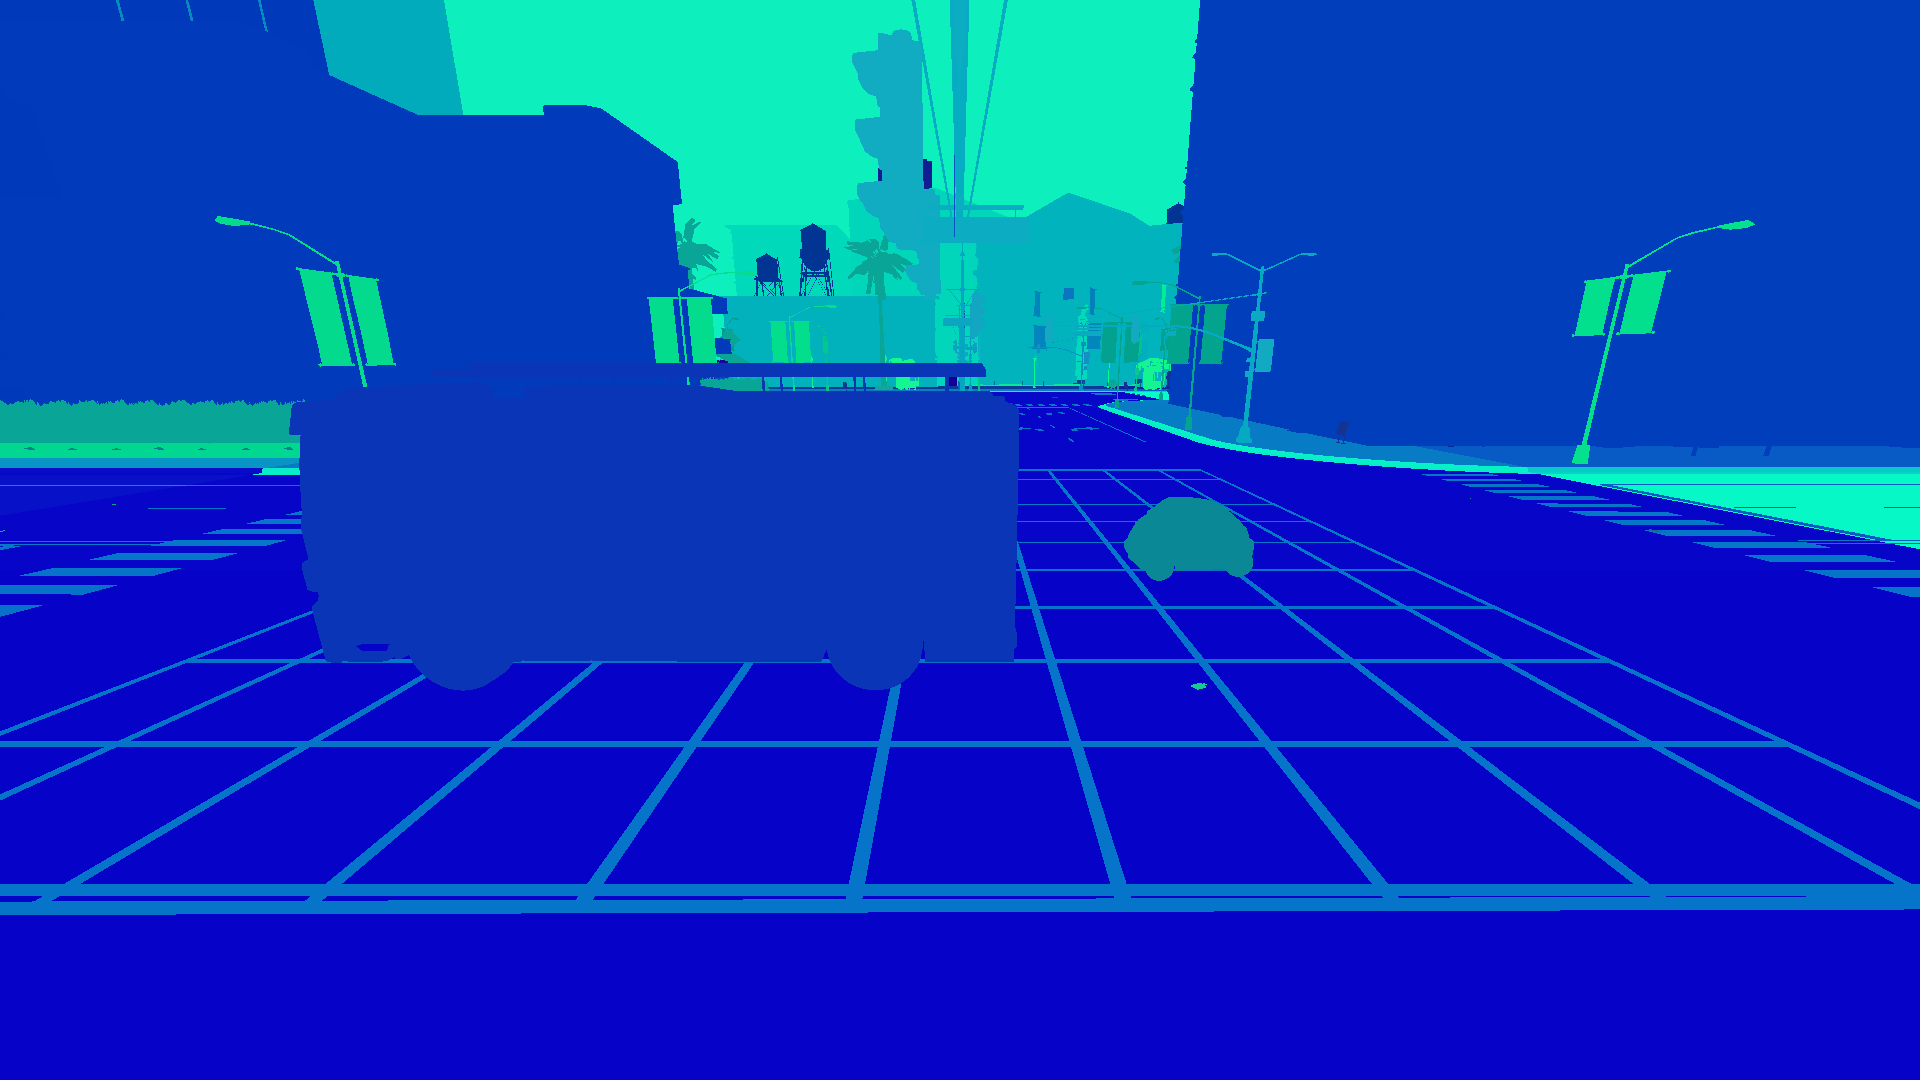
\includegraphics[width=0.5\textwidth]{images/instance_cam.jpg}}
  \caption[CARLA's cameras]{These two images display the difference between the output of the two camera types.} \label{fig:camera_outputs}
\end{figure}
%###################################################################################
%###################### Topic C             ########################################
%###################################################################################
\section{Related Work}
\chapter{Problem analysis} \label{problem_analysis}
\chapter{Approach for Solving the Issue} \label{approach}
% DELETEME: In this chapter you start addressing your actual problem. Therefore, it makes often sense to make a detailed problem analysis first (if not done in introduction). You should be sure about what to do and how. While writing in the background part, it might also make sense to include complex background information or papers you are basing on in this analysis. If you are solving a software problem, you should follow the state of the art of software development which basically includes: problem analysis, design, implementation, testing, and deployment. Maintenance is often also described but I believe this will not be required for most theses. Code should be placed in the appendix unless it is solving an essential aspect of your work.

This chapter provides an explanation of what techniques were used in the problem's solution. It is split into smaller subsections, which consider different parts of the proposed strategy.

\section{Organisation of the Simulation}
In general, to conduct real-world experiments is rather expensive and time-consuming, therefore we simulate different scenarios using CARLA. What is more, there are no limitations in the digital environment and data samples can be created faster without any distortions or noise. It offers an opportunity to implement and test different approaches and ideas in ideal conditions where no real-life restrictions exist.

Our simulation takes place in a realistic digital city "Town10HD\_Opt" from the CARLA assets package, which represents a whole town including, i.e., buildings, trees, traffic lights, parked vehicles, etc. The main location of the experiments is a junction of four roads, because, compared to other types of intersections, there exists a higher chance for accidents to happen, and an optimal camera placement is crucial for a safe mobility. On the junction's premises we place 3 CARLA objects from type Actor: 
\begin{itemize}
    \item 1 camera and 2 vehicles, which has the roles 'occluder' and 'target'
\end{itemize}
In pursuance of finding an optimal position for the camera sensor we consider the 4 angles of the region of interest (ROI) and also the points in the middle of each of the 4 edges like it is shown in Figure \ref{fig:camera_positions}. In this way, we earn an approximate idea which point or area has to be aimed for when placing a camera. Furthermore, this placement could be applied to other infrastructure of the same type, therefore it also guarantees flexibility and universality of the approach. 

With regard to the vehicles, which play the most important role in our research, we divide them into two categories:

\begin{itemize}
    \item \textbf{Occluder vehicle} - stays between the sensor and the target vehicle and covers some part of it because of its larger size or position regarding the sensor. For a realistic scenario we use a medium and large-sized vans or trucks, so that their shape generate a blind zone for the sensor's field of view, which then cannot recognize the occluded vehicle. 
    \item \textbf{Target vehicle} - is equal or smaller than the occluder, because we have to measure the degree to which it is occluded in various positions. If, for example, it has the bigger proportions, the chance of a camera not detecting it is quite decreased even if it stays behind the occluder. 
\end{itemize}
During the simulation we spawn both vehicles in different locations on the intersection in order to reproduce as many as possible static situations and decide whether an occlusion occurs or not.

\begin{figure} [h]
    \centering
    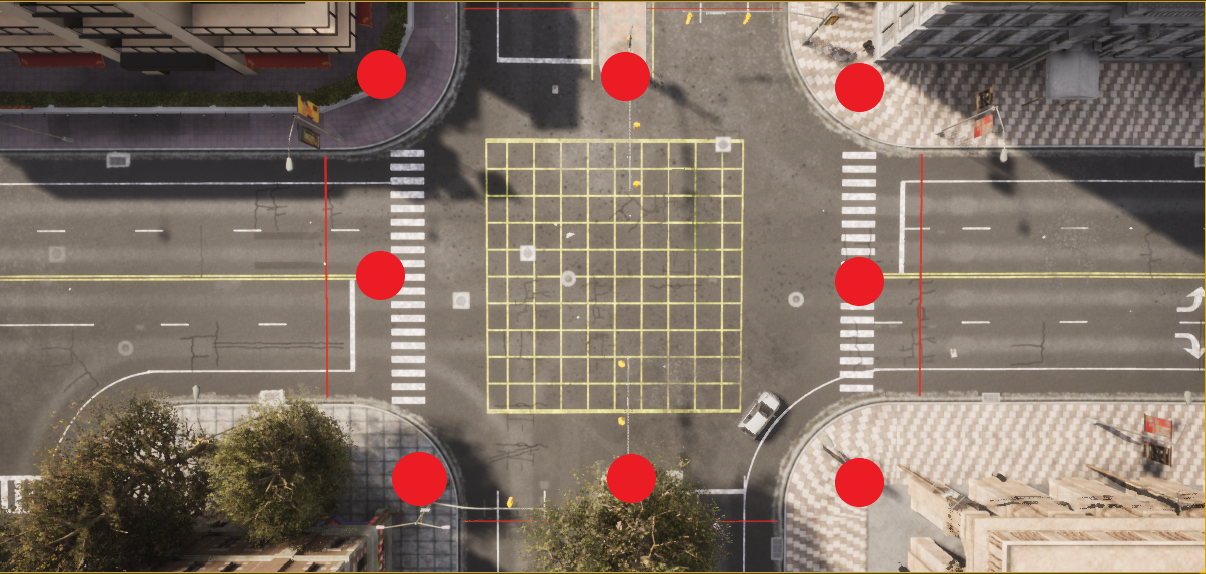
\includegraphics[width=\textwidth]{images/junction.png}
    \caption[Camera experiment positions]{This picture displays an example where the camera is going to be placed during simulations and shows the borders of our region of interest.}
    \label{fig:camera_positions}
\end{figure}

\section{Simulation Pipeline} \label{sec:sim_pipeline}

This thesis relies on a simulation pipeline for conducting experiments and evaluating their output, which consists of three main stages that can be seen on Figure \ref{fig:evaluation_pipeline}: 

\begin{enumerate}
    \item \textbf{Preparation of the experiment} - encompasses the configuration of all virtual world settings, as well as the creation of points on the test intersection that will be used during the experiments. In this stage a camera object is spawned within the simulated environment, which perceives the traffic and returns data that has to be evaluated. 
    \item \textbf{Reproduction of possible scenarios} - during this stage we have tuples of vehicles(occluder and target) that are spawned on the waypoints generated in the previous stage. In addition, after each new spawn, images from the camera are saved for further evaluation of the occlusion degree and the other metrics.
    \item \textbf{Evaluation of results} - being the last stage of the simulation pipeline, here the results are evaluated and used to generate a heatmap and a graph for a better visualisation, after which we discuss in \ref{evaluation} how our approach optimises traffic camera placement.
\end{enumerate}
In the following subsections we provide a more detailed explanation of how all the process from data generation via vehicles placement to output evaluation is realised.
\begin{figure} [h]
    \centering
    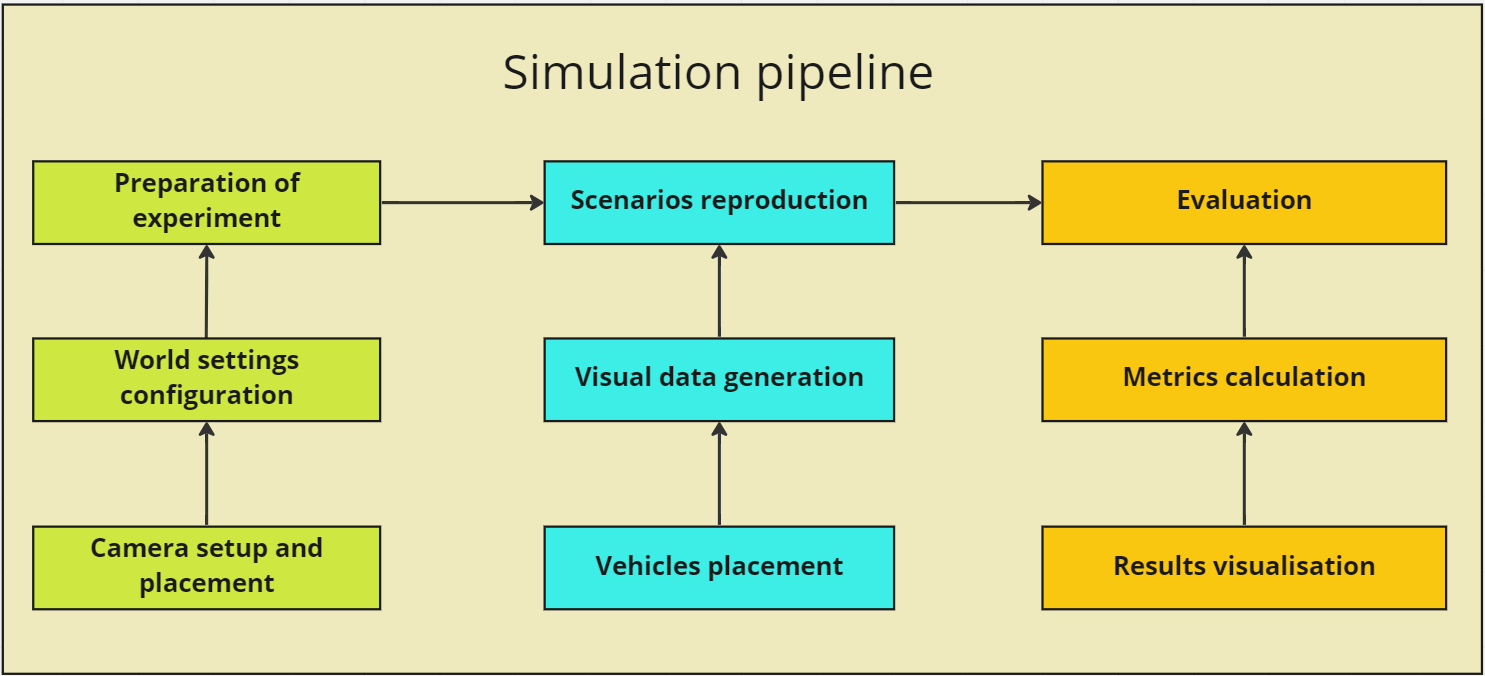
\includegraphics[width=\textwidth]{images/evaluation_pipeline.png}
    \caption[Evaluation pipeline]{This diagram represents schematically the simulation pipeline}
    \label{fig:evaluation_pipeline}
\end{figure}

\subsection{Experiment Setup and Environment Preparation}
As a prerequisite for each simulation it is important to adjust the world settings correctly in order to maintain a synchronous mode, which allows for reliable data from the sensors. In CARLA we set a client which communicates with our world and a traffic manager which is responsible for the behaviour of vehicles. 

When we are done with the creation of our simulated environment, the main priority is to generate waypoints within the intersection, which serve as spawn points for the vehicle actors. To clarify, all points belong to the road, where cars usually drive and no cases where a car spawns on the pavement or on a green area are considered. Furthermore, each point defines apart from the location also the direction in which the vehicle's head will point, therefore no situations like a car in the opposite direction or perpendicular to both driving directions occur in the experiments. For the purpose of covering maximal number of occlusion situations on the road we collect each existing waypoint in Figure \ref{fig:waypoints} that the simulator offers between the borders of the junction. On Figure \ref{fig:camera_positions} the ROI, defined by red borderlines, can be seen.

At the end of the preparation step we spawn a camera actor which should monitor all scenarios and perceive crucial for the research data. Therefore, cameras are positioned on such points, where they achieve maximal coverage of the region of interest and are able to avoid more potential occlusions. Each camera have adjustable parameter that are described in Table \ref{tab:camera_params}. In addition to these parameters, we define the camera tilt angle in a vertical plane, whose degree value is such that the camera field of view covers a bigger part of the intersection. 
\begin{table}[h]
\caption{Table for camera parameters and definitions used in this thesis\label{tab:camera_params}}
\centering
    \begin{tabular}{ | l | p{5cm} |}
    \hline
    Parameter & Definition  \\ \hline
    fov & Horizontal field of view in degrees. \\ \hline
    image\_size\_x & Image width in pixels. \\ \hline
    image\_size\_y & Image height in pixels. \\ \hline
    \end{tabular}
\end{table}

\begin{figure} [h!]
    \centering
    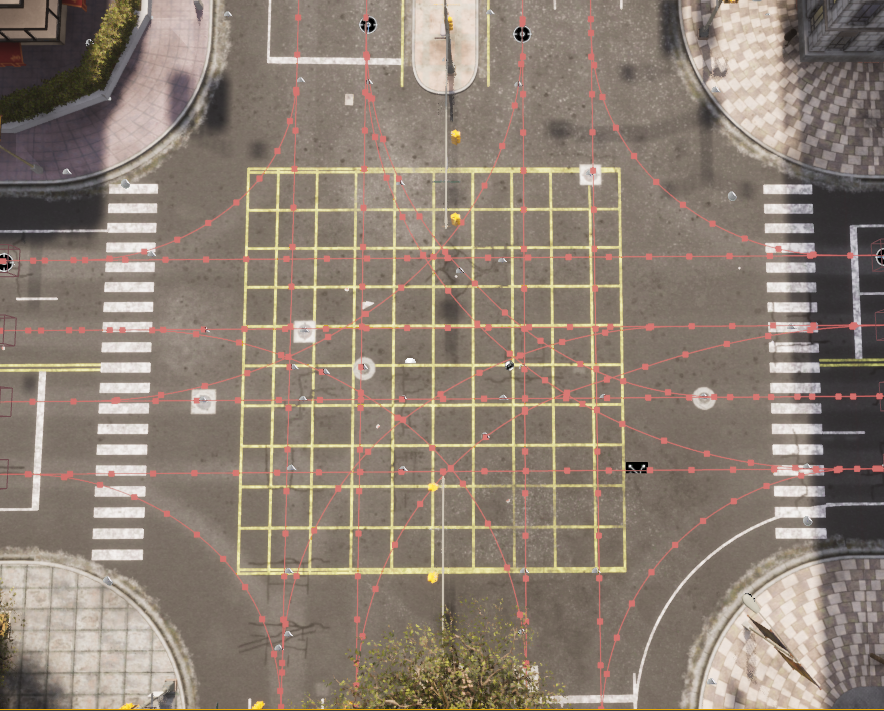
\includegraphics[width=0.7\textwidth]{images/waypoints.png}
    \caption[Intersection waypoints]{This picture illustrates all available spawn points for our vehicles}
    \label{fig:waypoints}
\end{figure}
\newpage

\subsection{Simulation of scenarios} \label{sec:sim_stage}
Many researches consider only static obstacles as occluder when executing their experiments and do not take into account the dynamic occlusion. Therefore, we follow the idea of \cite{occlusion_degree_model} and apply a similar approach in our work combined with static measurements. Like mentioned in \ref{sec:sim_pipeline} we use vehicles as actors for our experiments, which we spawn on previously generated waypoints. The idea of this strategy is to have two different by size vehicles, which are called an 'occluder' and a 'target', because we aim to reproduce the occlusion that happens each day in traffic. Autonomous vehicles require an accurate perception of the world around them to avoid accidents, which is why we recreate various scenarios by placing the vehicles on each pair of points. By doing so, we get the chance to recreate and analyse some occlusions, which could happen in a dynamic environment.

Vehicles in this work could not be placed on the same spawn point simultaneously and also positions, not included on the image plane, are not examined. Furthermore, depending on the waypoint there could be several directions for the vehicle, which also has impact on the volume of the blind zone caused by the larger vehicle. 

Due to the focus being on the occlusion degree, we have to know what percentage of the target vehicle is occluded. One way to overcome these problems is to use the bounding boxes of each vehicle, which are provided by the simulator. Our first idea was to convert all its eight vertices from the 3D world to the 2D image plane by choosing the upper-, lower-,  left- and rightmost points as exemplified with red points in Figure \ref{fig:bb_conversion}. Subsequently, we have an approximate 2D representation of the vehicle's borders and can subtract the visible part from the occluded car. However, after some experimentation with this strategy, it was asserted that this method is inefficient and unreliable. In comparison to the following approach, this one returns results with ca. 30-40\% difference from the correct and expected values. The main reason that justifies this behaviour is that a bounding box contains more points or pixels than these, which belong to the vehicle. Therefore, we needed another solution that calculates the occlusion precisely, which would be of utmost importance if later our approach is applied in a real-world scenario.
In our current implementation, due to the lack of depth information from a normal monocular camera, an instance segmentation camera (see \ref{instance_camera}) is applied instead of using an algorithm for object detection. The main advantages compared to previous method are mainly simplicity and accuracy, because this camera type provides us with ground-truth data in the form of an image, whose pixels have colour values according to the object each of them contain. It works like a 100\% accurate algorithm for object recognition, therefore it should be taken into account if the strategy is adopted by future works that depth information is a prerequisite for a reliable real-world implementation.

In order to calculate the correct percentage of occlusion, first is spawned the target vehicle, its number of pixels on the image plane are counted (see implementation in \ref{subsec:calc_occl}) and then the occluder is spawned. When both vehicles are present in the world, we can extract the part under occlusion. However, it is possible that in particular cases no occlusion exists, i.e., when the occluder is not positioned between the sensor and the target vehicle. In Figure \ref{fig:occlusion_views} it is shown how depending on the point of view an occlusion is either visible or does not occur. After each tuple of points is observed the implementation returns the following output, which is saved in a text file:
\begin{itemize}
    \item world coordinates of target vehicle (x, y, z)
    \item rotation of target vehicle (pitch, yaw, roll)
    \item occlusion degree given in percent
\end{itemize}

\begin{figure} [h!]
    \centering
    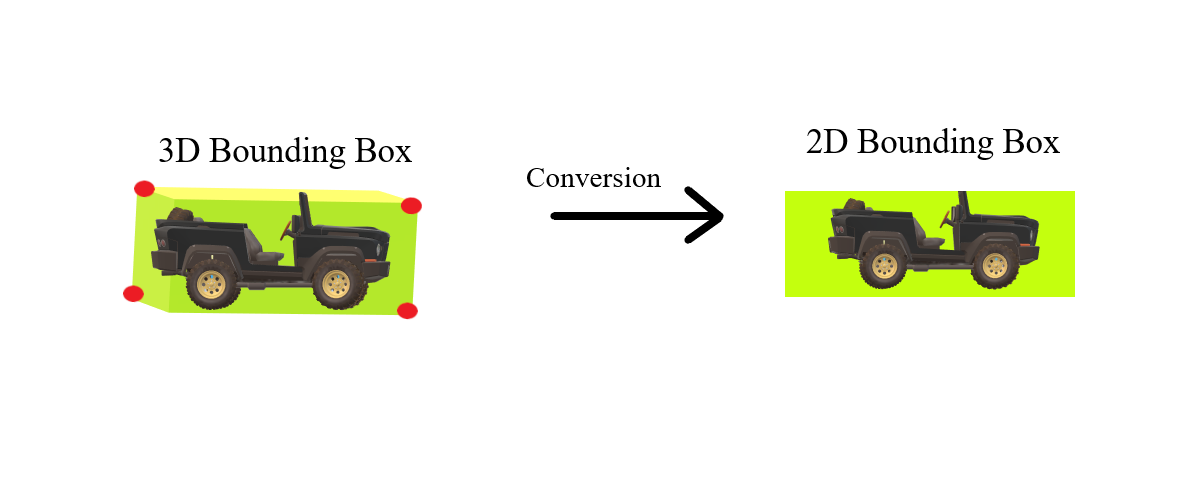
\includegraphics[width=0.8\textwidth]{images/2D_bounding_boxes.png}
    \caption[3D bounding box conversion]{On this illustration is shown the conversion from a 3D bounding box to a 2D one, which a camera would perceive.}
    \label{fig:bb_conversion}
\end{figure}

\begin{figure} [h!]
  \centering
  \subfloat[Occlusion from camera's point of view]{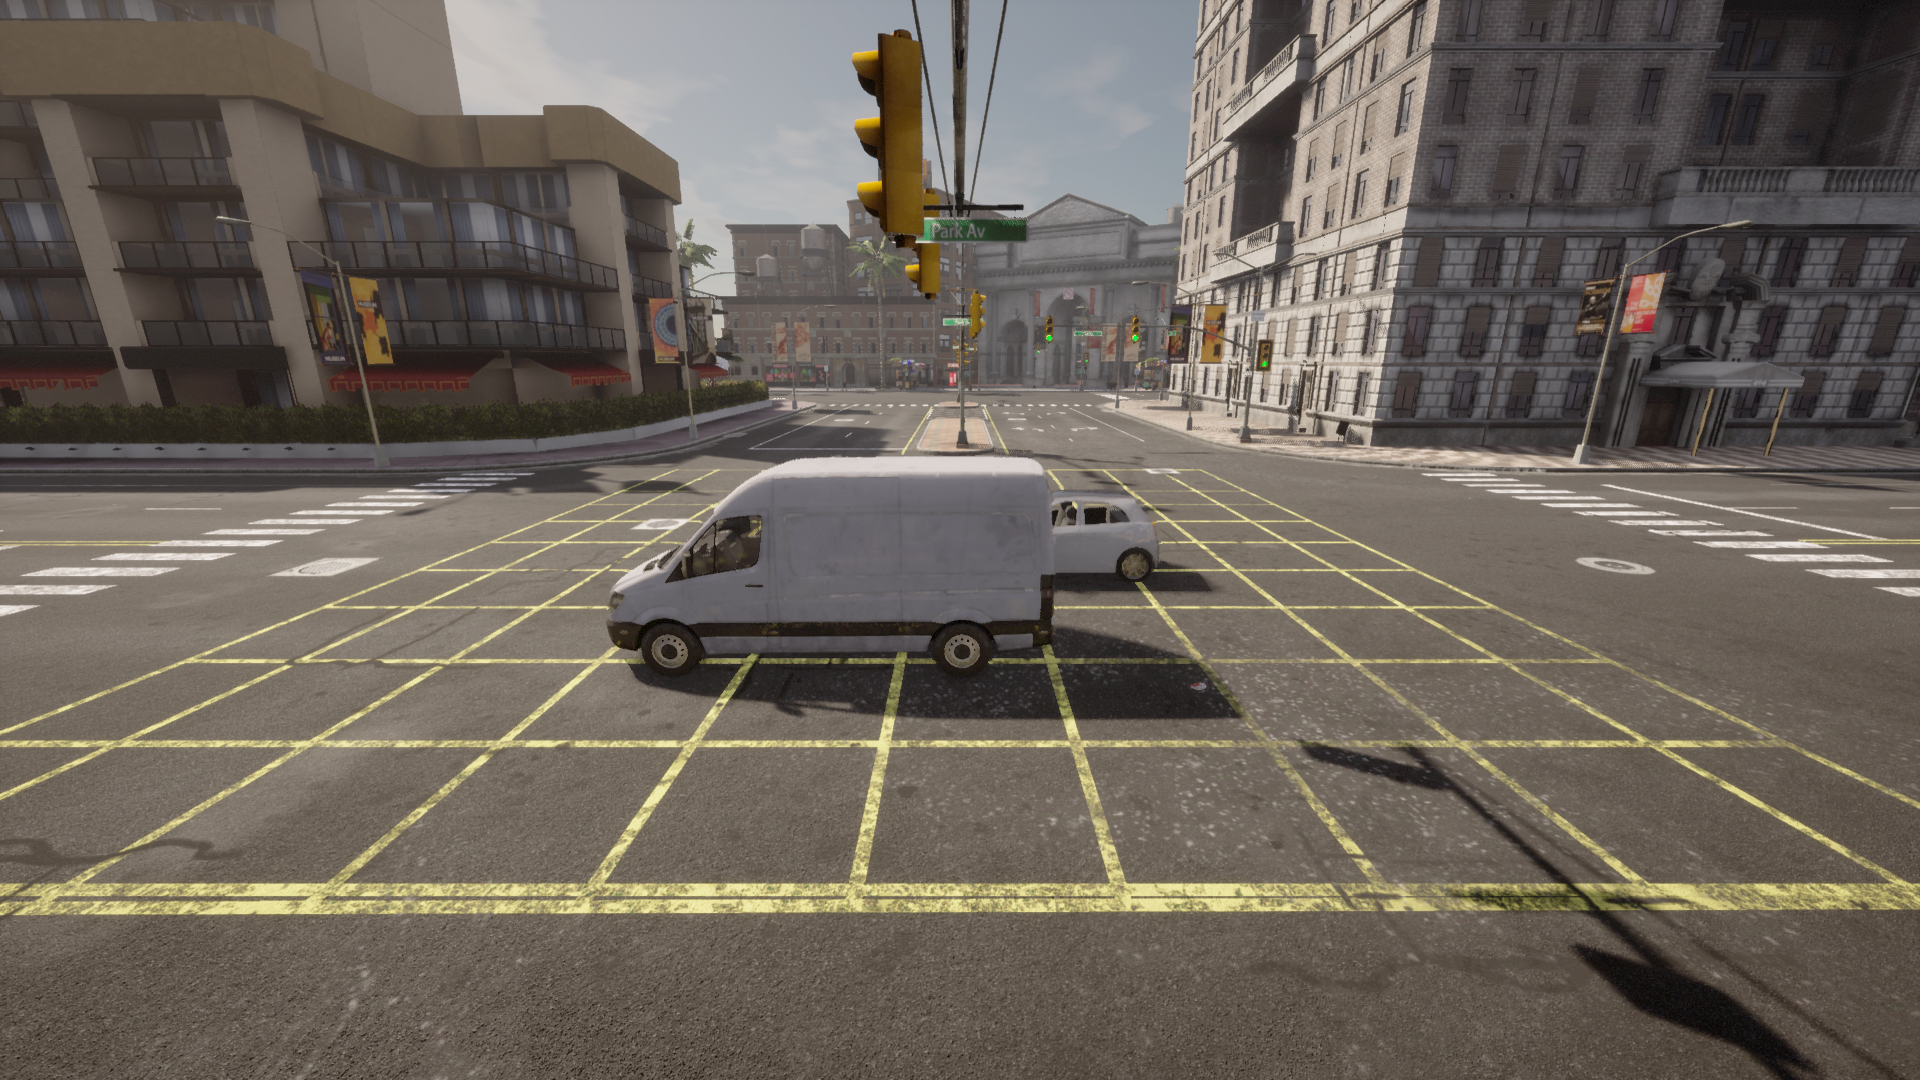
\includegraphics[width=0.574\textwidth]{images/camera_view_occlusion.jpg}}
  \hfill
  \subfloat[Occlusion from side point of view]{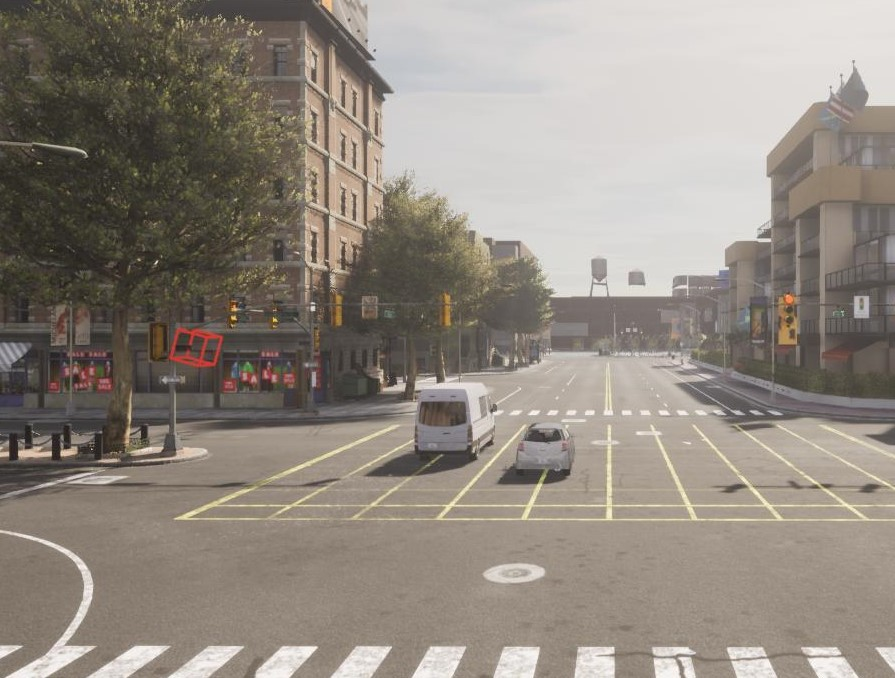
\includegraphics[width=0.426\textwidth]{images/different_view_occlusion.jpg}}
  \caption[Occlusion points of view]{These two images display how an occlusion is perceived from different points of view.} \label{fig:occlusion_views}
\end{figure}

\newpage
\subsection{Evaluation of Results}
When we already have the data from the simulation stage, it should be visualised for a better understanding of the results. In the evaluation stage, this thesis makes use of heatmap to illustrate where the occlusion occurs at most and thus choose the most optimal point of view for a camera. For the purpose of a coherent visualisation we discretise the intersection in equal rectangular blocks where each block has world X and Y coordinate values. Furthermore, to each of these blocks are assigned the positions where the target vehicle has been spawned. As mentioned in \ref{sec:sim_stage}, we receive an occlusion degree for each tuple of the junction's waypoints, which means that for a single position of the target we usually have more than one occlusion degree available. For this reason, during the generation of a heatmap for each saved spawn position in the result file, we calculate the average occlusion from all the values assigned to the position and display it on the map with an according colour from the colour palette. We use the heatmaps to explain whether the camera placement is optimal or not according to the amount of occlusion it detects, i.e., light colours imply that a little amount of occlusion was perceived whereas darker colours indicate loss of sight and an unfavourable sensor position.

In addition to the occlusion degree, we also rely on two metrics, which are inspired by \cite{occlusion_degree_model}, when comparing the performance of cameras placed on different locations. The first one estimates the ratio of times a target vehicle on a specific position is not detected by a camera because the occlusion percentage exceeds the particular threshold for object recognition to all times it has been on this location. Our second metric is the ratio of vehicles missed by the sensor in case they are out of its field of view to the total amount of traffic. When these two metrics have lower values, we are able to determine where is a reasonable area for camera installation, which will ensure a better traffic surveillance. 

\chapter{Implementation} \label{implementation}
This chapter describes how the approach we proposed in Chapter \ref{approach} is applied by using the Python API offered by CARLA. Moreover, we reveal the software implementation of the processes behind each of the three stages in our simulation pipeline.  

\section{Setup of Virtual Environment}
The simulation pipeline consists of three main stages - Data Generation for the experiments, Simulation of possible real-world scenarios and Evaluation of the results, as it was explained in the previous chapter. In the course of our first stage, we connect the client to the simulator's server, which represents the digital world for our research. The 3D simulator provides two options for a communication between client and server\footnote{\url{https://carla.readthedocs.io/en/latest/adv_synchrony_timestep/}, visited on 02/12/2022}:
\begin{itemize}
    \item \textbf{synchronous mode} - in this mode the client must notify via tick\footnote{Signal in CARLA for the server} when all the commands are prepared that the server is obliged to execute. This is the mode which is relevant for simulations where synchrony between, i.e., sensors and world is crucial. 
    \item \textbf{asynchronous mode} - this is the default mode, where the server runs the simulation as fast as possible and does not have to wait for a signal from the client, which ensures that everything is ready for the next step 
\end{itemize}

For this work the synchronous mode is set, because we require an environment, where we know location and rotation of world objects, receive accurate data from the camera and maintain a consistent connection to the server. When we enable the synchronous mode, we create a synchronous instance of the Traffic Manager, which handles any group of vehicles in the simulated world. For our experiments, we rely on the virtual city map "Town10HD\_Opt" and define good weather conditions, which do not affect the performance of the camera because we need optimal results in ideal conditions. Additionally, we remove the layer with parked vehicles, because otherwise they will be detected by the sensor and increase the number of pixels containing vehicles which are not important for the simulation.

\subsection{Sensor placement}
Having all synchrony-related settings adjusted, we then instantiate a new object of type Sensor from CARLA's blueprint library\footnote{\url{https://carla.readthedocs.io/en/latest/bp_library/}, visited on 03/12/2022}. This is a subtype of actor which can measure and stream data. For this thesis the sensor is instance segmentation camera which has the main parameters of each camera sensor: field of view, width and height of generated image. What is more, a sensor is responsible for perceiving data either whenever a new event is registered or on each tick-signal received from the client. This sensor in particular has a task to render all elements contained in the field of view with a specific colour according to their semantic tags (vehicle, building, traffic light, etc.) and a unique object ID assigned by the Unreal Engine at the moment of instantiation. 

With regard to the spawning of sensor, in CARLA one can attach it to a vehicle and thus to visualise an on-board point of view. However, the goal of this thesis is to find an optimal position in the infrastructure, therefore we spawn our traffic monitoring tool as displayed in Figure \ref{fig:camera_positions} on particular locations. Again, there is no algorithm for locations generation, they are completely random and aim to compare three points in each border of the region of interest, which makes eight in total. In order to receive data, which is then forwarded along the pipeline for examination, sensors have an integrated listening method. In short, there we provide as an argument a function that inserts every new image in a queue, which then can be accessed during the evaluation part. At the end, we define height, rotation and tilt angle of the camera so that it points to the intersection and have an unobstructed view. More information about what values for the camera's attributes are set for the experiments is described in chapter \ref{evaluation}.

\subsection{Waypoints generation}
The last step from the first stage is generation of waypoints suitable for our experiments, where pairs of vehicles are going to be placed to recreate real-world situations and estimate occlusion percentage, because it prevents the camera from a correct perception of the surrounding environment. CARLA supports methods\footnote{\url{https://carla.readthedocs.io/en/latest/core_map/}, visited on 03/12/2022}, which allow a user to select a landmark on the map and spawn an object there. In order to extract these points from the simulator, we have to specify which area is of interest. As we previously mentioned, we do not consider cases where a vehicle is spawned on impermissible places like pavements or green spaces. Therefore, the task of this work requires only valid road lanes as spawn location. Moreover, the simulated world offers the opportunity to choose from points which belong to possible driving routes and the process is the following one:
\begin{enumerate}
    \item The user gives a location as input and the simulator returns the nearest waypoint to it that lies on the premises of our region of interest, which in our case is an intersection of four roads.
    \item Knowing this waypoint, one can request from the simulator to return the junction which contains it.
    \item The returned junction comes with a list of various waypoints, therefore it should be specified in a method for extraction that we only need positions on driving lanes.
    \item In the previous step, we receive a list of pairs of points, which mark the beginning and the end of a lane. With a for-loop we iterate through all pairs and use a method from the simulator that returns a list of waypoints in the direction of the line a specified distance apart from each other. The new list contains all points from the current waypoint to the end of its lane.
\end{enumerate}
It is beneficial for the needs of our experiments to be able to define what distance should exist between the spawn positions. To illustrate an exemplary situation we use Figure \ref{fig:distance_waypoints}, where the distance between each point in a single lane is set to five meters. When the preparation of vehicle spawn locations is done, the simulation starts and the process is explained in the following section.

\begin{figure} [h!]
    \centering
    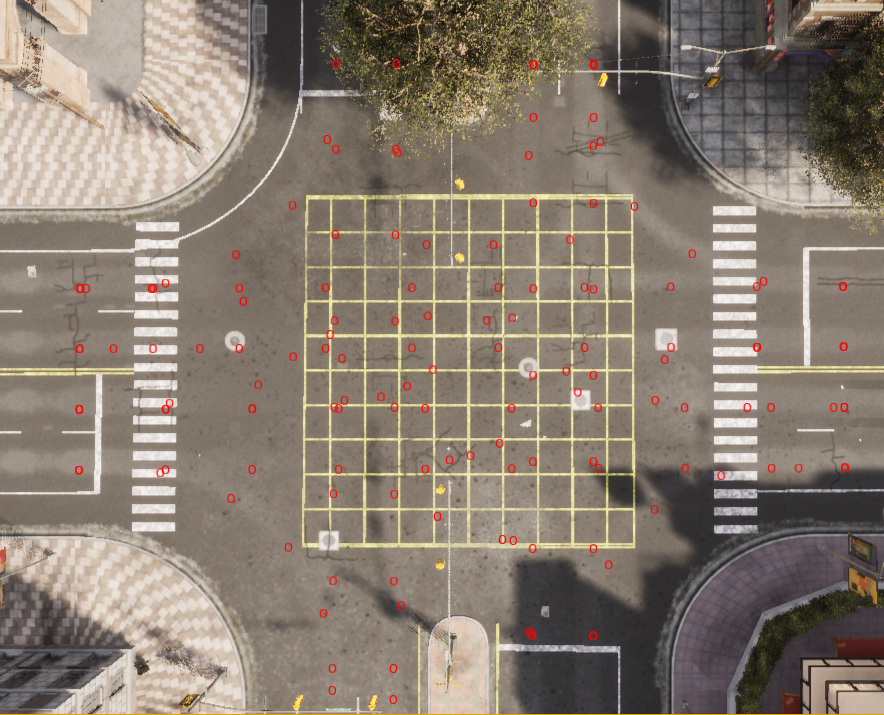
\includegraphics[width=0.75\textwidth]{images/waypoints_target.png}
    \caption[Vehicle waypoints with specified distance]{This image serves as an example of spawn points where we could place vehicles when the distance between them in each lane is 5 meters.}
    \label{fig:distance_waypoints}
\end{figure}

\section{Simulation of Valid Scenarios}
For the purpose of suggesting an optimal position for a camera sensor in the infrastructure that could enhance autonomous vehicles, improve communication between them and facilitate mobility per se, we have to reproduce real-world scenarios and observe how the sensor perform. The focus of this work is the occlusion, which occurs in everyday traffic when larger vehicles intercept a sensor's field of view, therefore we apply our own approach based on the Occlusion Degree Model proposed by Du et al. in \cite{occlusion_degree_model}. In subsection \ref{sec:sim_stage} we give a detailed explanation of how our experiments are designed, whereas here the technical means used by this stage are addressed.

\begin{figure} [h!]
    \centering
    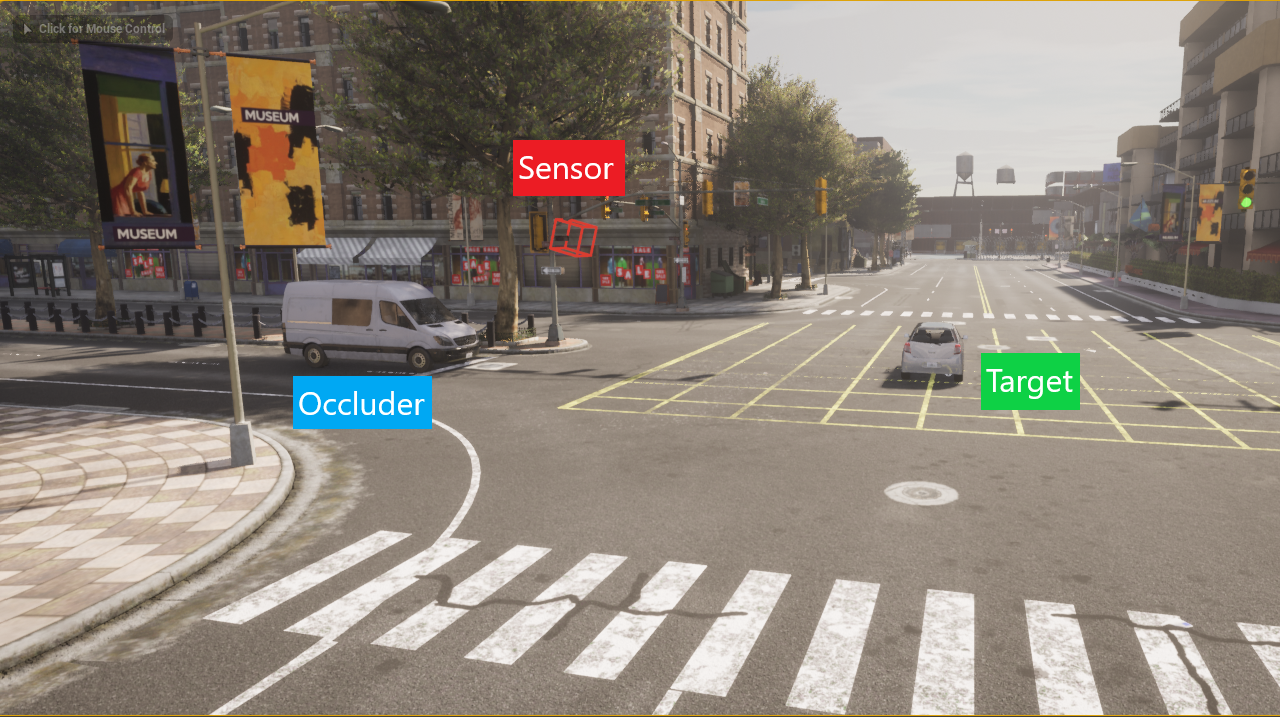
\includegraphics[width=0.85\textwidth]{images/behind_sensor.png}
    \caption[Vehicle spawned behind the camera]{We can see on this image a situation where the occluder is spawned out of the sensor's field of view, which makes it invisible for the sensor and is excluded from the experiment.}
    \label{fig:behind_sensor}
\end{figure}

\subsection{Spawning vehicles and their roles}
To start with, in each simulation we have two actor objects from type Carla.Vehicle, which can be chosen from the blueprint library\footnote{\url{https://carla.readthedocs.io/en/latest/bp_library/\#vehicle}, visited on 03/12/2022}. In this library a user can select whichever vehicle he needs for his purposes. In addition, vehicles are varying from motorcycles through small cars to large trucks. Again, our implementation inserts two vehicles in the virtual environment, which take the roles 'occluder' and 'target' depending on the vehicle's size. This means that if we put the label occluder to a vehicle 2x3m-sized vehicle and as a target vehicle we have a 4x8m-sized truck, it is certain that such scenario will be useless for experimental purposes, because in 95\% of the cases a normal object recognition algorithm would not have troubles in detecting it. For this reason, we suggest that always the occluder is larger than the target vehicle, which will guarantee more reliability of the results if this approach is to be adopted by further studies.

At the beginning, we generate a list of waypoints for both vehicles with a specified distance between them. Vehicles can only be spawned at the exact location of a waypoint and in the direction of the driving lane under them, which means that it is possible to spawn our actor on the same place multiple times but with different rotation. One important functionality of these waypoints is that the vehicle is always placed parallel to the ground and could not be hovering at an angle from thirty degrees, for example. Furthermore, this guarantees flexibility when simulating scenarios, because it is not necessary to always use a flat surface for the vehicles. 

Before placing the target on the first received waypoint, it is checked if the vehicle's centre is displayed on the image plane. The process is explained in subsection \ref{camera_model} and consists of several steps:
\begin{enumerate}
    \item World to camera matrix (W2C) generation - CARLA provides a method which returns the inverse matrix of the sensor as an array.
    \item Camera's intrinsic matrix $A$ generation - it contains the parameters of the sensor like coordinates of the principal point $u_0$ and $v_0$, skew index $\gamma=0$ (no distortion) and scale factors $\alpha$ and $\beta$ which have as a value the result of the focal length divided by the pixel size.
    \item 2D Projection of a 3D world point - we take the coordinates of the world point in an array, multiply it with the W2C matrix and change from Unreal Engine's coordinate system to a standard one $(x, y ,z) \rightarrow (y, -z, x)$. Afterwards, we multiply with the new array with the intrinsic matrix $A$ and both $x$ and $y$ are normalized by the third value in the array.
    \item If the final coordinates are negative or exceeds either the image's width or height then the vehicle is not spawned as it is practically invisible to the camera, and no occlusion could happen.
\end{enumerate}

When this check returns a positive output, the target vehicle is spawned in a height of 2 cm, as this is the minimum if we want the spawn to be successful, and then falls for some frames until it lands on the ground. We wait 20 frames until the physics are stabilised and the vehicle's z-coordinate remains constant. Then, we try to spawn the occluder vehicle on a location which is different from the target's one, because they cannot be spawned at the exact same point. We first check if the spawn point will cause an occlusion by:
\begin{enumerate}
    \item Measuring the diagonal of the occluder vehicle and taking only such positions where the distance between target and occluder spawn point is not longer than the diagonal. This guarantees mainly situations with occlusion, because we exclude positions where the occluder is far from the target and does not cover it. Furthermore, average truck's size is 3-4 meters, therefore it won't obstruct the sensor's view if it stays under it.
    \item Checking if the distance between sensor and occluder is longer than the one between sensor and target, which prevents the camera from considering spawn points behind the target vehicle.
\end{enumerate}
The above described constraints optimise simulations and reduce execution time significantly, because we consider mainly occlusion-prone points. Afterwards, it is checked again whether the occluder is visible for the camera, i.e. in Figure \ref{fig:behind_sensor} the Mercedes Sprinter is behind the sensor and would cause no occlusion, therefore it won't be considered in the experiment, but if that is not the case, the occluder successfully gets placed on the virtual intersection. During each iteration the camera records the situation on the road and streams data for evaluation of the occlusion, which is explained in the next subsection. Then the occluder is destroyed and simulation continues while the list with spawn points is not empty.

\begin{figure} [h!]
  \centering
  \subfloat[Vehicle at the moment of spawn]{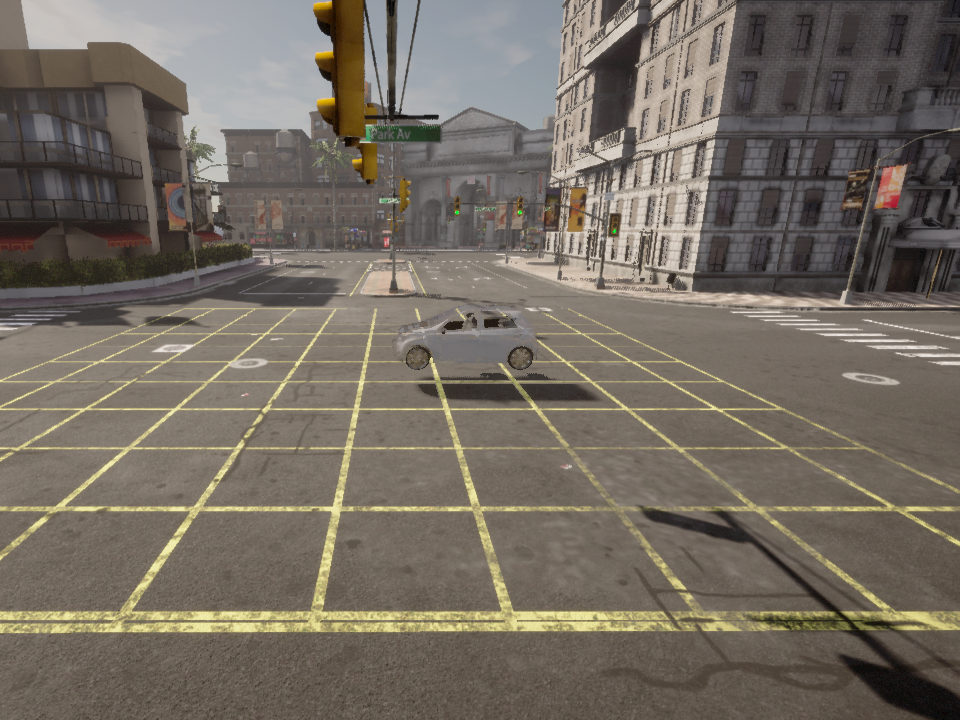
\includegraphics[width=0.5\textwidth]{images/spawn_air.jpg}}
  \hfill
  \subfloat[Vehicle on the ground]{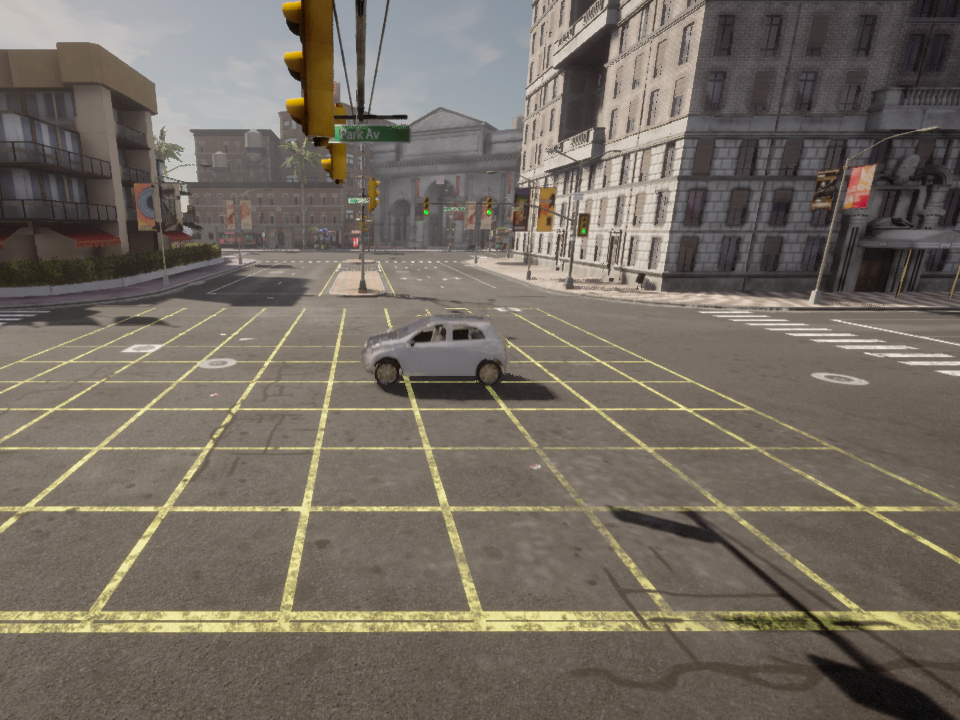
\includegraphics[width=0.5\textwidth]{images/spawn_ground.jpg}}
  \caption[Spawning a vehicle]{Both picture illustrate the described CARLA physics when a vehicle is spawned, it hovers first in the air and lands after some time on the ground.} \label{fig:spawn_vehicle}
\end{figure}

 \subsection{Camera output and occlusion calculation} \label{subsec:calc_occl}
 In this work the instance segmentation camera is used as a reliable sensor that provides only ground-truth data. An important advantage of this type of camera is that it can perform better than an object recognition method. However, it is still under development by the CARLA creators and has one drawback that after we spawn the target vehicle, we have to wait several ticks until it's displayed on the image plane. This happens because, as mentioned in the previous subsection, in the simulator a vehicle is always spawned in the air, therefore it needs some time to land on the ground and the world's physics to be stabilised as shown in Figure \ref{fig:spawn_vehicle}. Nevertheless, this issue does not cause any delays for the simulation.
 
 To calculate the occlusion, we need an image of the target vehicle alone and an image where both vehicles are available in the world. Therefore, the first image is taken after the target vehicle is spawned and when it already stays stationary on the ground. Subsequently, we try to spawn the occluder and take the image with both vehicles available in the simulator if it was successful. In the performed experiments, we do not wait for the occluders to be fully stationary, but only to be visible on the image plane, because this will increase execution time. This means, that the occlusion measured is no more than one percent higher than the real one. Again, result's accuracy is not heavily affected by this issue. For the calculation we use the following help methods:
 \begin{itemize}
     \item \textbf{Conversion of raw image data to a 2D array} - the data that is output by a camera is in a raw format, which should be transformed into a 2D array so that we could iterate through all pixels. This method extracts the blue, green and red values for each pixel and puts them in the exact row and column as the location of the pixels on the image plane. Blue and green channels define the object's unique ID, and the red one assigns it to a class according to its type.
     \item \textbf{Calculation of pixels containing a specific label} - in CARLA each item has a tag which defines the type of the object, e.g., whether it is a vehicle a building or something else. This method calculates how many pixels contain a given object type using the information from the red channel. 
 \end{itemize}

With the first help method we are able to generate arrays which we can iterate through, while the second one tells us how many pixels represent the target vehicle in an image, when the occluder is absent. We then iterate through the 2D array and consider only rows whose pixels contain objects from type vehicle. Inside each row we inspect again only columns containing a vehicle and calculate the ID of a vehicle using the blue and green value of a pixel. An important point to be made is that Unreal Engine gives an ID to each object spawned in the 3D world, which is not always the result of the expression \ref{eq:instance}, where B represents the blue value and G the green one.
When the ID crosses the hexadecimal value of $0\times10000$ which comprises 65536 in a decimal number system, we have to subtract this value from the object's ID so many times as it is contained in it, which is shown in the equation \ref{eq:new_id}.

\begin{equation}B + G * 256\label{eq:instance}\end{equation}

\begin{equation}\textrm{new\_ID} \: = \textrm{ID} - \lfloor \textrm{ID} / 65535 \rfloor * 65536\label{eq:new_id}\end{equation}

After we are done with the described calculations, we check if the occluder's ID equals the converted blue and green channels' values and increment the number of target's visible pixels. If we have reached a situation where the visible numbers are equal to all pixels from the first image, meaning the vehicle is not occluded, we break the loop and return the occlusion, which comprises the result of equation \ref{eq:occlusion}. In Figure \ref{fig:occlusion_calc} an example of two pictures used for estimation of the occlusion are provided, where the occlusion on the second one is 75\% and at this point exists a higher chance that the target vehicle is not detectable. Apart from the occlusion, the location of the target vehicle is also included in a text document after each iteration. 
% At the end of the simulation, we also add the number of times a vehicle was not visible on the camera and therefore not spawned to the document, which is crucial for the evaluation stage.  

\begin{equation}
    \frac{\textrm{target\_max\_pixels} - \textrm{target\_visible\_pixels}}{\textrm{target\_max\_pixels}} * 100 \label{eq:occlusion}
\end{equation}

\begin{figure} [h!]
  \centering
  \subfloat[Single target vehicle]{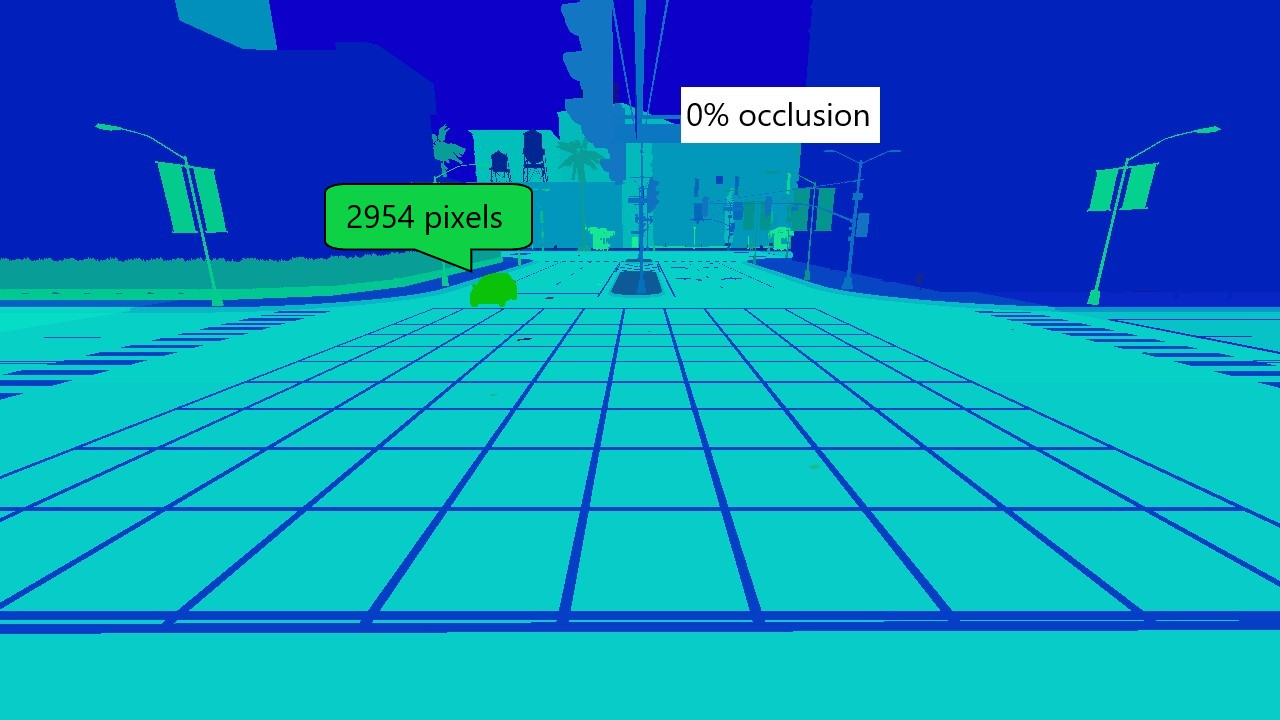
\includegraphics[width=0.5\textwidth]{images/before_occlusion.jpg}}
  \hfill
  \subfloat[Both occluder and target vehicles]{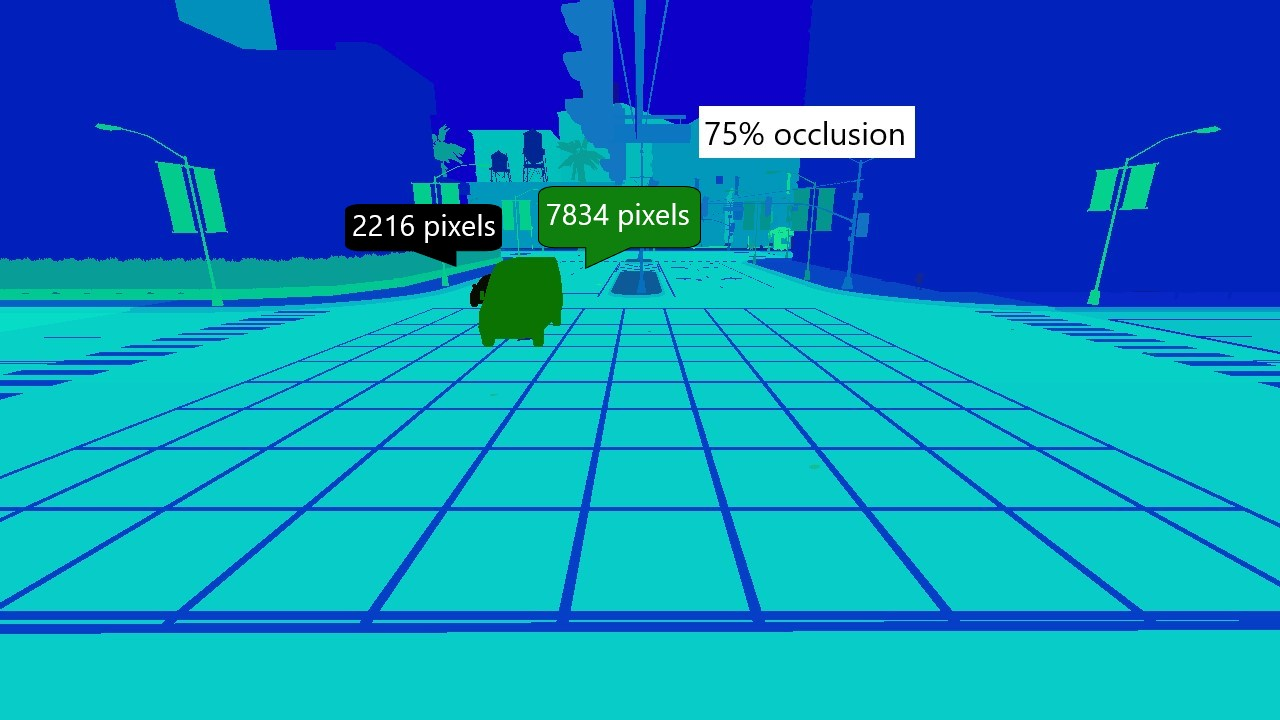
\includegraphics[width=0.5\textwidth]{images/after_occlusion.jpg}}
  \caption[Calculation of an occlusion]{The two images represent how vehicles are seen through the instance segmentation camera. On the right picture there is an occlusion of 75\%, visible pixels of each vehicle are shown in bubbles above them.} \label{fig:occlusion_calc}
\end{figure}
 
 \section{Evaluation of Results}
 In the final step of our simulation pipeline, we scrutinise our results to get an impression of which positions offer a more optimal sensor's performance. Due to the fact that our results are saved in a text file, we need some way of data visualisation, therefore heatmaps are chosen as the most suitable technique for displaying traffic data, i.e., in the studies \cite{heatmap_first, heatmap_second} also rely on heatmaps for their results. We mentioned previously that each row in the text file contains X and Y coordinates of a target's spawn location, as well as the occlusion degree. In order to display the results correctly on the heatmap, we first divide our region of interest - the intersection - into equal-sized $M \times N$ blocks where $M,N \in \mathbb{N}_{>0}$, so that we get a set of blocks denoted by $S$. Furthermore, the coordinates of a location are assigned to a block $B_{x,y} \in S$, which should represent the intersection's area on the heatmap. With regard to the heatmap's dimensions, they are defined by the absolute value of the difference between the minimum and maximum value of each coordinate, so that it contains all available spawn points from the ROI:
 \begin{equation}
     |x_{max} - x_{min}| + 1 = M
 \end{equation}
 \begin{equation}
     |y_{max} - y_{min}| + 1 = N
 \end{equation}
 
 Heatmaps require a 2D array, which they could read the information from. Additionally, dimensions of arrays cannot be negative values. In Unreal Engine's 3D world coordinates sometimes contain a negative value, which is problematic for the previous statement, and therefore we avoid this issue by converting each value accurately to a non-negative one using the following technique:
 \begin{enumerate}
     \item Find the minimal value $X_{min}$ among the X-coordinates in the list and round it, because we need non-decimal values for a heatmap's coordinates. In our case all x-coordinates have negative values.
     \item Take its absolute value $|X_{min}|$, iterate through each X-value and increment it with the absolute value. This step sets the lowest X-coordinate to be a starting point of the heatmap array. For example, if $X_{min} = -50$, each value will be then incremented by $50$.  
     \item Repeat steps 1 and 2 for each Y-coordinate value.
 \end{enumerate}
 In case the min-coordinates are positive numbers, we take their value with a minus sign in front of it and add it to each X and Y value respectively, so that the heatmap begins at $(0,0)$. For example, if $X_{min} = 5$, each X-coordinate will be decreased by $5$.
 
\begin{figure} [h!]
    \centering
    \includesvg[width=0.85\textwidth]{images/6m_target_heatmap.svg}
    \caption[Heatmap target full occlusion]{This image illustrates an example of how a heatmap would look like when the distance between waypoints is 6 m and the occlusion is 100\% on each location.}
    \label{fig:heatmap_target}
\end{figure}
 
\subsection{Occlusion degree and metrics} \label{subsec:metrics}
Our main criterion for an efficient position of a camera is when a low occlusion degree is estimated in the examined positions. During the simulation of occlusion-prone situations for our pair of vehicles, we can receive multiple values for a single target location, therefore we take the highest occlusion value for each point when generating the heatmap. For a comparison, we also provide a heatmap that contains the average occlusion from all values found in the text file for each single spawn point (see equation \ref{eq:avg_occl}). However, we do not consider the lack of occlusion when calculating the average occlusion.  

\begin{equation}
    \textrm{avg\_occlusion\_degree} = \textrm{sum\_of\_occlusion\_for\_current\_location} / \textrm{location\_occurences}\label{eq:avg_occl}
\end{equation}

When we calculate the occlusion degree, we set the value in a 2D array on the position $\textrm{array}[y,x]$. The reason for changing the order of coordinates is that the Python data visualisation library Seaborn\footnote{\url{https://seaborn.pydata.org/}, visited on 04/12/2022} we use is based on Matplotlib\footnote{\url{https://matplotlib.org/}, visited on 04/12/2022}, which reads first the y-dimension of the array and then the x-dimension, e.g., if we have an occlusion 40\% for the location $(x=12,y=5)$, then we have to request the element on position $(5,12)$ from the array. When everything is set correctly in the array, we plot the result using the "YlGnBu" (yellow-green-blue) colour palette, which displays the low values using light yellow colour and dark blue colour for the higher ones. We can see in Figure \ref{fig:heatmap_target} how the results for each target location at 6 m distance from each other are presented when there is a full occlusion everywhere. 

Apart from the occlusion, we also have two metrics, which are responsible for a better estimation of the experiment data. Our goal is to find a camera position, which minimises the score of the two metrics. In a real-life scenario it is impossible for a monocular camera to detect each vehicle in its field of view, when another vehicle has occluded it, which increases the chance for accidents to happen, e.g., if a truck stays in front of a small car, then the camera won't be able to detect the car and will act if it does not exists. For this reason, we want to have the minimum number of undetected vehicles due to a high occlusion degree (see M1). In addition, our motivation for the second strategy is to be able to avoid as many occlusions perceived by the camera as possible, and if this cannot happen to only have a few locations in the region of interest where this phenomenon occurs (see M2). We list our metrics below.

M1 - Undetected Vehicles due to a High Occlusion. It calculates the ratio of all times the occlusion exceeded a previously specified threshold $T$ to all times an occlusion greater than $0\%$ was detected. For a camera to be efficient, it is necessary that we get a low value for the tested position.
\begin{equation}
   M1 = \frac{\sum\textrm{occlusion}_{T}}{\sum\textrm{occlusion}_{>0}}
\end{equation}

M2 - Occlusion Occurrences Ratio. In order to calculate this metric, we collect information from the text file for each target position observed. We divide the times when an occlusion has occurred to all the times when we spawned a pair of vehicles and performed a calculation. To clarify, we strive again towards low values for each sensor placement configuration. Although, our constraints when spawning an occluder increases the number of collision-prone situations, we still monitor cases where no occlusion exists.  

\begin{equation}
    M2 = \frac{\sum\textrm{occlusion}_{>0}}{\sum\textrm{occlusion}_{>=0}}
\end{equation}

In this chapter we described how our approach is implemented, how we execute the simulations and what metrics do we consider when comparing the output of camera on each position, placed on different locations. Discussion and presentation of our results are provided in the following chapter.
\chapter{Experiments and Evaluation}
\label{evaluation}
% DELETEME: The evaluation chapter is one of the most important chapters of your work. Here, you will prove usability/efficiency of your approach by presenting and interpreting your results. You should discuss your results and interpret them, if possible. Drawing conclusions on the results will be one important point that your estimators will refer to when grading your work.

This chapter serves as a presentation of the actors used in our experiments, and the output of the camera, after which is discussed if it has met the expectations and whether the approach was efficient in providing a solution for the CPO problem.

\section{Experiments}
In this thesis, two different experiments were conducted in order to evaluate the performance loss of cameras. What is more, with the help of heatmaps and using the metrics M1 and M2 we are able to define an optimal camera position. The experiments aim to check if problems from Chapter \ref{problem_analysis} are handled efficiently by the proposed strategy. In the next subsections, we inform about the laptop used for our simulations and explain into details each experiment. Afterwards, we discuss the results and the efficiency of our metrics.

\subsection{Technical specifications}
The following list contains technical specifications of the machine, which all experiments were simulated on:
\begin{itemize}
    \item \textbf{Processor} - Intel Core i7-10750H CPU 2.60GHz
    \item \textbf{RAM} - 16 GB DDR5
    \item \textbf{GPU} - NVIDIA GeForce RTX 3060 6 GB
    \item \textbf{SSD} - 1 TB
\end{itemize}

\newpage
\subsection{First experiment - change height and angle of camera}
The main objective of our first experiment is to evaluate the performance of cameras at different height, because we concluded from the found literature in Chapter \ref{problem_analysis} that there is little information about which height is optimal for traffic surveillance. We use heatmaps to present the maximal occlusion degree for each spawn point. Additionally, our metric M2 is applied in order to see what part from all cases were occlusions and choose these positions which have scored lower values. During the execution of simulations, we rely on a camera with the following configurations:
\begin{itemize}
    \item FoV (horizontal angle) = $80^{\circ}$
    \item Resolution = $1280\times720$ pixels or also known as 720p
\end{itemize}
The reason for our horizontal angle is that we wanted to cover as much as possible from our region of interest and an average traffic surveillance camera on the market has a horizontal field of view $70^{\circ} - 110^{\circ}$. In a real-world scenario, a wider field of view will cause a fisheye effect\footnote{When an image is distorted by stretching the picture around a rounded camera lens} to occur and has to be taken into account. However, in our experiments the conditions are ideal and we do not apply image distortion. We have 8 enumerated positions for the camera, which can be seen in Figure \ref{fig:positions_enumerated}, where we place it at a pre-defined height. On each of these spawn locations for our sensor, we define 6 levels for the height beginning at 5 meters and going up to 10 meters with a 1-meter step. This results in 48 simulations, where we set $0^{\circ}$ for the tilt angle at 5 meters, $-10^{\circ}$ at 6 meters and then reach up to $-30^{\circ}$ at 10 meters with a $-5^{\circ}$ step. In this way, we guarantee that the camera has approximately the same sight over the vehicles and the blind spot under the sensor does not increase. The region of interest, which comprises the four-road intersection, is limited by the red lines in Figure \ref{fig:positions_enumerated} and is used in each of the two experiments.

During each simulation, we generate a list with waypoints for the target vehicle that are 3 meters apart and one for the occluder, but with 1-meter distance between spawn points. We decided to use Seat Leon (see Fig. \ref{fig:seat_leon}) as a target and Jeep Wrangler Rubicon (see Fig. \ref{fig:jeep_wrangler}) as an occluder for our scenarios, because in an urban area people mainly utilise normal cars or SUVs for their transportation needs, and therefore it is more often the case that these two types of vehicles are captured by a camera. In our second experiment, we consider pairs of vehicles of different type in order to broaden the variety of measured occlusions.

\begin{figure} [h!]
    \centering
    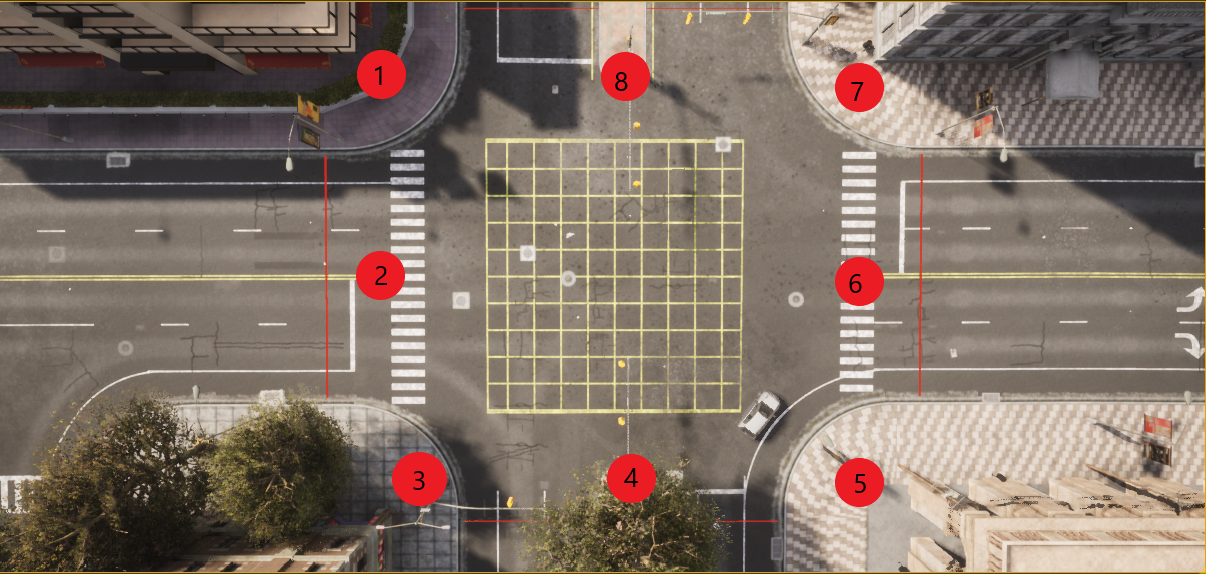
\includegraphics[width=0.90\textwidth]{images/positions_numerated.png}
    \caption[Enumerated camera positions]{This image shows the number of each camera's position examined in our simulations.}
    \label{fig:positions_enumerated}
\end{figure}

\newpage
\subsection{Second experiment - change threshold for target vehicle recognition}
In our second experiment our goal is to observe how strong the occlusion is when there are different types of vehicles. Here we use the same parameters for the camera, but this time it is placed only at 8 meters above the ground. The reason behind this decision is that we have mentioned in Section \ref{main_problems} that the minimum for an ideal height is exactly 8 meters. Furthermore, we guarantee same conditions for all sensor positions by setting their tilt angle at $-20^{\circ}$ in order to have an accurate comparison. For this scenario, we use three pairs of vehicles and execute a simulation for 6 camera positions, which comprises a total of 18 simulations, 6 of which are also part of the first experiment. Moreover, we decided to not consider positions 4 and 8 here, because their view is obstructed by the traffic lights and hanging signs on their poles, therefore their range of view is limited.

For this experiment we rely on the pairs:
\begin{itemize}
    \item Seat Leon and Jeep Wrangler Rubicon
    \item Ford Mustang and Mercedes Sprinter (see Figures \ref{fig:ford_mustang} and \ref{fig:mercedes_sprinter})
    \item Ambulance truck (see Fig. \ref{fig:ambulance}) and Mercedes Sprinter
\end{itemize}
Our idea is to reproduce three possible traffic scenarios, in which we have a normal car and SUV, a normal car and a large van, as well as two large-sized vehicles. In this way, we can ensure that a variety of vehicles' sizes are covered by this study. Important to mention is that the distance between target spawn points is again set to 3 meters. 

For the purpose of assessing optimal camera locations, we apply our M1 metric for a priori specified threshold. In the real world it is vital for a camera to miss as little as possible objects, which were hidden due to other large-sized vehicles. Therefore, we set an occlusion tolerance threshold, after which the target vehicle is no more detectable, to 50\%, 75\% and 90\%. By implementing this constraint, we can conclude from the score of our metric how many occlusions from all the detected ones could actually blind the camera. Finally, we choose these positions, which output the lowest values. Apart from the metric, heatmaps display the maximum occlusion degree for each target position, captured by the sensor.

%###################################################################################
%###################### Results             ########################################
%###################################################################################
\section{Results}\label{results}
In the heatmaps and tables below, we can inspect the results from both experiments. In order to maintain a well-arranged visualisation of the output, we are going to present only the heatmaps for 5 and 10-meter height and compare the impact of increasing elevation on the maximum occlusions. For our second experiment, we will visualise the results from cameras placed at 8 meters above the road in positions 1, 3 and 6. The other heatmaps are placed in the appendix 
\ref{appendix_heatmaps}, if one wants to analyse them.

\subsection{First experiment} \label{subsec:first_exp_heat}

\begin{figure}[!htb]
\minipage{0.5\textwidth}
  \includesvg[width=\linewidth]{images/position0/pos0_5m.svg}
  \caption{Pos.1 at 5 m height}\label{fig:pos1_5m}
\endminipage\hfill
\minipage{0.5\textwidth}
  \includesvg[width=\linewidth]{images/position0/pos0_10m.svg}
  \caption{Pos.1 at 10 m height}\label{fig:pos1_10m}
\endminipage\hfill
\end{figure}

\newpage
\begin{figure}[!ht]
\minipage{0.5\textwidth}
  \includesvg[width=\linewidth]{images/position1/pos1_5m.svg}
  \caption{Pos.2 at 5 m height}\label{fig:pos2_5m}
\endminipage\hfill
\minipage{0.5\textwidth}
  \includesvg[width=\linewidth]{images/position1/pos1_10m.svg}
  \caption{Pos.2 at 10 m height}\label{fig:pos2_10m}
\endminipage\hfill
\end{figure}

\begin{figure}[!ht]
\minipage{0.5\textwidth}
  \includesvg[width=\linewidth]{images/position2/pos2_5m.svg}
  \caption{Pos.3 at 5 m height}\label{fig:pos3_5m}
\endminipage\hfill
\minipage{0.5\textwidth}
  \includesvg[width=\linewidth]{images/position2/pos2_10m.svg}
  \caption{Pos.3 at 10 m height}\label{fig:pos3_10m}
\endminipage\hfill
\end{figure}

\begin{figure}[!ht]
\minipage{0.5\textwidth}
  \includesvg[width=\linewidth]{images/position3/pos3_5m.svg}
  \caption{Pos.4 at 5 m height}\label{fig:pos4_5m}
\endminipage\hfill
\minipage{0.5\textwidth}
  \includesvg[width=\linewidth]{images/position3/pos3_10m.svg}
  \caption{Pos.4 at 10 m height}\label{fig:pos4_10m}
\endminipage\hfill
\end{figure}

\newpage
\begin{figure}[!ht]
\minipage{0.5\textwidth}
  \includesvg[width=\linewidth]{images/position4/pos4_5m.svg}
  \caption{Pos.5 at 5 m height}\label{fig:pos5_5m}
\endminipage\hfill
\minipage{0.5\textwidth}
  \includesvg[width=\linewidth]{images/position4/pos4_10m.svg}
  \caption{Pos.5 at 10 m height}\label{fig:pos5_10m}
\endminipage\hfill
\end{figure}

\begin{figure}[!ht]
\minipage{0.5\textwidth}
  \includesvg[width=\linewidth]{images/position5/pos5_5m.svg}
  \caption{Pos.6 at 5 m height}\label{fig:pos6_5m}
\endminipage\hfill
\minipage{0.5\textwidth}
  \includesvg[width=\linewidth]{images/position5/pos5_10m.svg}
  \caption{Pos.6 at 10 m height}\label{fig:pos6_10m}
\endminipage\hfill
\end{figure}

\begin{figure}[!ht]
\minipage{0.5\textwidth}
  \includesvg[width=\linewidth]{images/position6/pos6_5m.svg}
  \caption{Pos.7 at 5 m height}\label{fig:pos7_5m}
\endminipage\hfill
\minipage{0.5\textwidth}
  \includesvg[width=\linewidth]{images/position6/pos6_10m.svg}
  \caption{Pos.7 at 10 m height}\label{fig:pos7_10m}
\endminipage\hfill
\end{figure}

\newpage
\begin{figure}[!htb]
\minipage{0.5\textwidth}
  \includesvg[width=\linewidth]{images/position7/pos7_5m.svg}
  \caption{Pos.8 at 5 m height}\label{fig:pos8_5m}
\endminipage\hfill
\minipage{0.5\textwidth}
  \includesvg[width=\linewidth]{images/position7/pos7_10m.svg}
  \caption{Pos.8 at 10 m height}\label{fig:pos8_10m}
\endminipage\hfill
\end{figure}

\begin{table}[!h]
\caption{This table presents the M2 score of each camera position at different height level \label{tab:height_experiment}}
\centering
    \begin{tabular}{ | c | c | c | c | c | c | c | c | c |}
    \hline
    Height & Pos.1 & Pos. 2 & Pos. 3 & Pos. 4 & Pos. 5 & Pos. 6 & Pos. 7 & Pos. 8 \\ \hline
    5 m & 0.50 & 0.49 & 0.70 & 0.52 & 0.54 & 0.55 & 0.74 & 0.68\\ \hline
    6 m & 0.49 & 0.48 & 0.66 & 0.45 & 0.53 & 0.53 & 0.73 & 0.63\\ \hline
    7 m & 0.47 & 0.48 & 0.65 & 0.49 & 0.51 & 0.52 & 0.71 & 0.64\\ \hline
    8 m & 0.48 & 0.47 & 0.63 & 0.48 & 0.51 & 0.50 & 0.68 & 0.61\\ \hline
    9 m & 0.48 & 0.46 & 0.61 & 0.44 & 0.50 & 0.49 & 0.63 & 0.58\\ \hline
    10 m & 0.46 & 0.44 & 0.57 & 0.33 & 0.47 & 0.46 & 0.61 & 0.55\\ \hline
    \end{tabular}
\end{table}

\newpage
\subsection{Second experiment}

\begin{figure}[!htb]
\minipage{0.5\textwidth}
  \includesvg[width=\linewidth]{images/position0/pos0_8m.svg}
  \caption{Pos.1 Seat and Jeep}\label{fig:pos1_8m}
\endminipage\hfill
\minipage{0.5\textwidth}
  \includesvg[width=\linewidth]{images/mustang_sprinter/sprinter_mustang_pos0.svg}
  \caption{Pos.1 Ford and Mercedes}\label{fig:pos1_ford_merc}
\endminipage\hfill
\end{figure}

\newpage
\begin{figure}[!htb]
\minipage{0.5\textwidth}
  \includesvg[width=\linewidth]{images/sprinter_ambulance/ambulance_sprinter_pos0.svg}
  \caption{Pos.1 Ambulance and Mercedes}\label{fig:pos1_amb_merc}
\endminipage\hfill
\minipage{0.5\textwidth}
  \includesvg[width=\linewidth]{images/position2/pos2_8m.svg}
  \caption{Pos.3 Seat and Jeep}\label{fig:pos3_8m}
\endminipage\hfill
\end{figure}

\begin{figure}[!htb]
\minipage{0.5\textwidth}
  \includesvg[width=\linewidth]{images/mustang_sprinter/sprinter_mustang_pos2.svg}
  \caption{Pos.3 Ford and Mercedes}\label{fig:pos3_ford_merc}
\endminipage\hfill
\minipage{0.5\textwidth}
  \includesvg[width=\linewidth]{images/sprinter_ambulance/ambulance_sprinter_pos2.svg}
  \caption{Pos.3 Ambulance and Mercedes}\label{fig:pos3_amb_merc}
\endminipage\hfill
\end{figure}

\begin{figure}[!htb]
\minipage{0.5\textwidth}
  \includesvg[width=\linewidth]{images/position5/pos5_8m.svg}
  \caption{Pos.6 Seat and Jeep}\label{fig:pos6_8m}
\endminipage\hfill
\minipage{0.5\textwidth}
  \includesvg[width=\linewidth]{images/mustang_sprinter/sprinter_mustang_pos5.svg}
  \caption{Pos.6 Ford and Mercedes}\label{fig:pos6_ford_merc}
\endminipage\hfill
\end{figure}

\newpage
\begin{figure}[!htb]
\minipage{0.5\textwidth}
    \includesvg[width=\linewidth]{images/sprinter_ambulance/ambulance_sprinter_pos5.svg}
  \caption{Pos.6 Ambulance and Mercedes}\label{fig:pos6_amb_merc}
\endminipage\hfill
\end{figure}

\begin{table}[!htb]
\caption{This table presents the M1 score at 8 m height for a specified threshold and vehicles Seat Leon and Jeep Wrangler Rubicon\label{tab:jeep_seat_threshold}}
\centering
    \begin{tabular}{ | c | c | c | c | c | c | c |}
    \hline
    Threshold & Pos. 1 & Pos. 2 & Pos. 3 & Pos. 5 & Pos. 6 & Pos. 7 \\ \hline
    50\% & 0.17 & 0.22 & 0.06 & 0.11 & 0.17 & 0.09\\ \hline
    75\% & 0.02 & 0.06 & 0.01 & 0.01 & 0.03 & 0.0\\ \hline
    90\% & 0.0 & 0.0 & 0.01 & 0.0 & 0.0 & 0.0\\ \hline
    \end{tabular}
\end{table}

\newpage
\begin{table}[!htb]
\caption{This table presents the M1 score at 8 m height for a specified threshold and vehicles Ford Mustang and Mercedes Sprinter\label{tab:ford_merc_threshold}}
\centering
    \begin{tabular}{ | c | c | c | c | c | c | c |}
    \hline
    Threshold & Pos. 1 & Pos. 2 & Pos. 3 & Pos. 5 & Pos. 6 & Pos. 7 \\ \hline
    50\% & 0.38 & 0.48 & 0.39 & 0.36 & 0.44 & 0.41\\ \hline
    75\% & 0.24 & 0.31 & 0.21 & 0.18 & 0.26 & 0.22\\ \hline
    90\% & 0.15 & 0.18 & 0.12 & 0.12 & 0.14 & 0.12\\ \hline
    \end{tabular}
\end{table}

\begin{table}[!htb]
\caption{This table presents the M1 score at 8 m height for a specified threshold and vehicles Ambulance Truck and Mercedes Sprinter\label{tab:amb_merc_threshold}}
\centering
    \begin{tabular}{ | c | c | c | c | c | c | c |}
    \hline
    Threshold & Pos. 1 & Pos. 2 & Pos. 3 & Pos. 5 & Pos. 6 & Pos. 7 \\ \hline
    50\% & 0.08 & 0.15 & 0.08 & 0.07 & 0.12 & 0.09\\ \hline
    75\% & 0.0 & 0.0 & 0.0 & 0.0 & 0.0 & 0.0\\ \hline
    90\% & 0.0 & 0.0 & 0.0 & 0.0 & 0.0 & 0.0\\ \hline
    \end{tabular}
\end{table}

%###################################################################################
%###################### Discussions         ########################################
%###################################################################################
\newpage
\section{Discussions}\label{discussions}
In this section we are going to analyse the above displayed heatmaps and tables in order to compare camera's performance in various situations and decide which positions brought the most optimal results. Furthermore, we discuss which height levels were beneficial to the efficiency of our visual sensor.

\subsection{Results of first experiment}
To start with, if we examine the heatmaps from Subsection \ref{subsec:first_exp_heat} and Table \ref{tab:height_experiment}, then we can assert that height is actually of utmost importance for the quantity of detected occlusions. For instance, in Figure \ref{fig:pos1_5m} and Figure \ref{fig:pos1_10m} it is noticeable that the difference of 5 meters significantly decreases the degree of occlusion for each target's spawn location. We are also able to see that our tilt angle is set correctly according to the height and ensures that the same spawn positions remain visible for the camera and new ones also appear at 10 meters. In Figure \ref{fig:pos1_8m} there are still some occlusions higher than 80\%, which still does not achieve the goal we are looking for. 

Out of all positions, there are two offering a lower performance than the other ones - positions 4 and 8. The reason for this behaviour is that there are traffic lights and street signs hanging from the poles, which obstruct their view of the whole region of interest. Moreover, this setback also deprives them of detecting locations on the road, which results in less evaluated situations, as can be asserted from heatmaps \ref{fig:pos4_5m} and \ref{fig:pos8_5m}. However, this outcome proves that our check for points out of the camera's field of view works properly and could also be applied to future experiments for a real-world scenarios.

For this study, it is of interest that an optimal camera position detects fewer occlusions, therefore we used our metric M2 to evaluate which location is efficient for the task. In the table \ref{tab:height_experiment} it makes directly an impression that positions 1 and 2 have scored the lowest values at 5-meter height. However, if we take into account the M2 score of positions 4 and 8, they seem to outperform some other locations, which is not the case. As we mentioned previously, when a sensor is placed there its FoV is limited and sees half the spawn points, which should be in fact recognisable for it. For this reason, their scores will be only valid, if the same amount of target points are available on the image plane. Another important point to be made after examining the table is that with the increase of height, the number of occlusion decreases, which is to be expected due to the fact that the sensor's view angle to the vehicles changes and can monitor them from an unhindered point of view in comparison to the lower heights. At 5, 6 and 7 meters our camera does not show a significant difference in the number of detected occlusions between the test pair of vehicles, whereas over 8 meters the sensor tends to identify with 10-15\% fewer occlusions. With the output of our first experiment, we can consider the statement that an ideal height for a traffic camera starts at 8-meter (see \ref{main_problems}) height as correct.

Finally, after inspecting the heatmaps and the M2 score for each camera placement, positions 1, 2, 3 and 7 guarantee a wider field of view compared to the others, because they have had a larger number of target spawn points in their sight during the experiment. Regarding the quantity of occlusion which is displayed on the heatmap at 10-meter height, position 3 seems to avoid them more efficiently, but its M2 score is the third highest in the table, which means that 57\% of all calculations were occlusions. Nevertheless, this metric is not that accurate when comparing the score at a certain height for different positions, because some positions detect more points around the target vehicle, which allows for more non-occlusion situations and thus the smaller score. In conclusion, we can say that higher placement is crucial, because there are almost no physical view obstructors. Additionally, wider range of view implies better perception of the environment, like it is guaranteed by positions 1, 2, 3 and 7.

\subsection{Results of second experiment}
During this experiment were different types of vehicles involved, which led to a better overview how size of the occluder affects the received quantity of occlusion. For example, when we compare heatmaps \ref{fig:pos1_8m} and \ref{fig:pos1_ford_merc}, it is clear that a camera at the height of 8 meters has a more obstructed view when a Mercedes Sprinter stays in front of a Ford Mustang than in the case when a Jeep Wrangler Rubicon is placed between the sensor and the target vehicle. This ensuing performance we explain by the fact that a Mercedes Sprinter is $2,5-3 m$ tall and for this reason a larger blind zone is formed behind it. Moreover, independent of camera's position this phenomenon occurs in each of the simulations at the height of 8 meters, therefore it is reasonable to place a camera on at a higher level above the road, otherwise the sensor will be less efficient in its tasks.

If we look at Figures \ref{fig:pos6_8m} and \ref{fig:pos6_amb_merc} we notice that there is only a slight difference in the detected occlusion degree, which is due to approximately the same size of the pair of vehicles. What we find surprising in position 6 is that the Mercedes Sprinter has caused less occlusion of the ambulance truck in comparison to the other occluder, but in our opinion the larger size of the trucks is to blame for it. To provide further explanation, more pixels on the image plane represent the ambulance truck as opposed to the Seat Leon, therefore the occlusion degree by the first vehicle increases slower. Nevertheless, if we consider the results from the other heatmaps, it seems that problematic for the sensor are only cases where the occluder vehicle is taller than the target one.

Apart from the heatmaps, we also applied our M1 metric for this experiment in order to investigate what part of all detected occlusions are the ones that exceed a pre-defined threshold. To start with, from Table \ref{tab:jeep_seat_threshold} we realise that in positions 3 and 7 were detected less than 10\% of occlusions, whose degrees were above 50\%. In a real-world situation, 50\% occlusion should not burden an object recognition algorithm, but still to have less severe occlusions monitored is our objective. Subsequently, in the third row the occlusion degrees above 90\% for each position is between 0 and 1\%, which is expected due to the near sizes of both Seat Leon and Jeep Wrangler Rubicon. What is more, it is a rare case that same-sized vehicles cause a full view obstruction to each other, when a camera is placed at least 8 meters above them.

However, if we have a look at Table \ref{tab:ford_merc_threshold}, the values change considerably, as there have been calculated more than 35\% occlusions whose degrees were above 50\%. According to the results, camera positioned at 8 meters is not reliable because it detects numerous occlusions, when we have trucks or vans on the street. Out of all positions 3, 5 and 7 offer a promising performance even in such environmental conditions. On the contrary, positions 2 and 6 tend to suffer more efficiency loss than the other locations, which is due to their rather central position and field of view. As it is illustrated by the heatmaps \ref{fig:pos6_5m} and \ref{fig:pos2_5m}. the number of target spawn points that have been detectable from the camera is low.

Finally, in Table \ref{tab:amb_merc_threshold} we notice that little occlusion occurs between the large-sized vehicles when the threshold is 50\% and above 75\% no occlusion was recorded by the camera, which is an optimal result in case of big vehicles crossing a junction. Taking everything into consideration, positions 3, 5 and 7 have scored the lowest M2 values, which mean they perform well independent of the vehicles' sizes and types.

After having examined and analysed the results of both experiments in detail, we can advance the opinion that positions 3 and 7 outperform the other ones and offer a balance between perceived number of spawn locations and occlusion degree. Definitely, cameras on a higher level (min. 8 m) above the ground have an increased visibility over the road and decrease the blind zone caused by taller vehicles. 

\subsection{Efficiency of metrics}
As we have seen in the previous subsections, two metrics (M1 and M2) were essential for arriving at a decision about which position and which height contribute to an enhanced camera efficiency. Their role in our approach, as described in Section \ref{subsec:metrics}, was to distinguish which occlusions were greater than a pre-defined threshold and to calculate how many out of all examined situations delivered an occlusion. After we have analysed the results, it can be assumed that they fulfilled their task and aided us in determining areas where a camera performs promisingly. However, there were two drawbacks that arose:
\begin{enumerate}
    \item M2 is appropriate, when one investigates the behaviour of camera at a different height on the same position. When the tilt angle is adjusted like in our experiments, a camera can see an identical number of spawn points, because the FoV does not change. If, however, we want to compare positions 3 and 4, we will see in Table \ref{tab:height_experiment} that the second one output lower values, which could lead us to a wrong conclusion about the two positions. Therefore, heatmaps were also involved in the data visualisation, which implied that position 4 has observed 50\% fewer spawn locations and in this way the M2 score gets unreliable. For the purpose of avoiding this issue, it is advisable to extend the metric and compare as well the number of monitored spawn points when studying two positions. Thus, it is ensured that the value of the metric is not influenced by side aspects.
    \item M1 is responsible for evaluating what part of all situations that resulted in occlusion denotes a value which exceeds a threshold for object recognition. Overall, it was accurate and served its role, but does not bring valuable information, as it can be seen at the second two rows in tables \ref{tab:jeep_seat_threshold} and \ref{tab:amb_merc_threshold}, when vehicles of the same size are compared. In our case, cameras were placed at 8 meters above the vehicles, from where it is impossible to detect occlusions larger than 80-90\%. However, if we consider the scenario in Table \ref{tab:ford_merc_threshold} where the occluder is significantly taller than the target vehicle, M1 provides useful data, because more occlusions land in the sensor's range of view. Therefore, instead of applying the M1 metric for same-sized vehicles at the same height, it is reasonable to compare the change in performance at different height levels and using a truck as occluder. In this way, worst-case scenarios can be examined, which is important for generating precise results for a real-world implementation. 
\end{enumerate}

\chapter{Conclusion and Future Work}
\label{conclusion}
%#############################################################
%###################### Summary   ############################
%#############################################################
\section{Summary}
% DELETEME: put a plain summary of your work here. Summaries should be made of each Chapter beginning with Chapter~2 and ending with you evaluation. Just write down what you did and describe the corresponding results without reflecting on them.
In this work, we started by reflecting on important scientific information as background for understanding the solution we propose. Additionally, we mentioned various studies in the area of camera placement optimisation, described their strategies for solving the issue and explained that the ODM of Du et al. in \cite{occlusion_degree_model} served as inspiration for our approach. Afterwards, in Chapter \ref{problem_analysis} we outlined main problems found in the literature during our research. Information about which height should be aimed for and little number of view-obstructors in an experiment are the issues this thesis was concerned with. In order to investigate which camera positioning is optimal, we presented an approach, which included a 3D simulator as testing environment, two test vehicles and an instance segmentation camera. Moreover, the meaning behind our experiments was to see which out of 8 randomly chosen positions is efficient in detecting less occlusions. To provide an insight into our implementation, Chapter \ref{implementation} described in detail which functionalities of CARLA were used and how our simulation pipeline works, which consists of 3 stages - Data generation, Experiment conduction, Result Evaluation. At the end of the fifth chapter, we discussed two metrics for comparison of cameras' performance, where the focus is on the number of detected occlusions and those which exceeded a certain threshold (see Section \ref{subsec:metrics}). During the evaluation part, we chose heatmaps and tables to visualise the results, then analysed them and drew a conclusion that positions 3 and 7 outperform the other ones by taking scores from both metrics M1 and M2 into consideration.

%#############################################################
%###################### Conclusion ###########################
%#############################################################
\section{Conclusion}
% DELETEME: do not summarize here. Reflect on the results that you have achieved. What might be the reasons and meanings of these? Did you make improvements in comparison to the state of the art? What are the good points about your results and work? What are the drawbacks?
Our approach was successful in determining positions for an efficient traffic camera and defining 8 meters as a minimal height. In comparison to studies like \cite{total_coverage_optimum} and \cite{max_camera_coverage} our strategy involved considering static occlusion in many spawn locations and in this way we provide an enhanced generic approach, which is applicable everywhere. Another benefit of our work is that impact of height on camera was tested, which showed that a higher position detects fewer occlusions and have a more accurate view over the road. What is more, in our implementation we used CARLA's instance segmentation camera, which generates ground-truth data and eliminates the necessity of an object detection algorithm. However, if our proposal is to be involved in real-world experiments, depth information should be available and also an algorithm for object recognition must be integrated, because there will be a difference compared to the simulated environment where each object ca n be accessed. Although our simulations try to approximate dynamic occlusion, they still remain in the area of static experiments. In our experiments, the distance between target vehicle spawn locations is 3 m which can be decreased to 0.5 m, if a dynamic scenario has to be represented accurately. What is more, for such shorter distance our algorithm will be slow, especially when large-sized vehicles participate. 

%#############################################################
%###################### Future Work ##########################
%#############################################################
\section{Future Work}
% DELETEME: Regarding your results - which problems did you not solve? Which questions are still open? Which new questions arose? How should someone / would you continue working in your thesis field basing on your results?

After inspecting the results, we were able to solve the two issues we discussed in the problem analysis. Nevertheless, our approach is focused only on static occlusion and ground truth data, while still lacking some necessary factors for plausible camera performance. For instance, in the future it can be extended by using more vehicles in the simulations in order to observe how traffic density affects object detection and occlusion occurrences. Having mentioned object detection, it is important to implement one of the latest algorithms to see how much time a camera needs to notice a vehicle and combined with our M1 metric it can be realised above what occlusion degree a vehicle is no more visible. By now, we have results for only one camera, therefore further ones can be added to increase the field of view and decrease occlusion by having different points of view. The last suggestion would be to implement some camera constraints as severe weather conditions or image distortion, which will be responsible for reproducing a real-world behaviour.

%__________________________End_of_Thesis______________________________________________
\cleardoublepage
\addcontentsline{toc}{chapter}{Bibliography}
%harvard citations style, please uncomment harvard package in the usepackage area
%\bibliographystyle{agsm}
%remove the following line when using harvard style citation
%\bibliographystyle{plainnat}
\bibliographystyle{unsrt}
%specify bibtex file here
\bibliography{input/mybib}
%add appendix to TOC
\addcontentsline{toc}{chapter}{Appendices}
\chapter*{Appendices}
\label{appendices}
DELETEME: everything that does not fit into your work, e.g. a 5 page table that breaks the reading flow, should be placed here

%###################################################################################
%###################### Appendix A          ########################################
%###################################################################################
%\newpage
\addcontentsline{toc}{section}{Appendix A: Abbreviations}
\section*{Appendix A: Abbreviations}
\begin{center}
\begin{tabular}{ll}
\textbf{FoV}	&	Field of View\\
\textbf{LiDAR}	&	Light Detection and Ranging\\
\textbf{ODM}	&	Occlusion Degree Model (mathematical model)\\
%\textbf{abk}	&	erklärung\\
%\textbf{abk}	&	erklärung\\
%\textbf{abk}	&	erklärung\\
%\textbf{abk}	&	erklärung\\
%\textbf{abk}	&	erklärung\\
%\textbf{abk}	&	erklärung\\
%\textbf{abk}	&	erklärung\\
%\textbf{abk}	&	erklärung\\
%\textbf{abk}	&	erklärung\\
%\textbf{abk}	&	erklärung\\
%\textbf{abk}	&	erklärung\\
\end{tabular}
\end{center}

%###################################################################################
%###################### Appendix B          ########################################
%###################################################################################
\newpage
%change this
\addcontentsline{toc}{section}{Appendix B: {\LaTeX} Help}
\section*{Appendix B: {\LaTeX} Help}
%remove this
%###################################################################################
%###################### HowTo               ########################################
%###################################################################################
\subsection*{How to Use This Template}
\begin{itemize}
\item Remove all of my text which is mostly labeled with DELETEME
\item Change the information in the 00a\_title\_page.tex file
\item Use the information written in this section
\item Ask you supervizor to help you
\item If I am not your supervizor and noone else can help you, write me an email (aubrey.schmidt@dai-labor.de)
\end{itemize}

%###################################################################################
%###################### Citations           ########################################
%###################################################################################
\subsection*{Citations}
Citing is one of the essential points you need to do in you thesis. Statements not basing on results of your own research\footnote{in what ever context} not being cited represent a breach on the rules of scientific working. Therefore, you every statement needs to be cited basing on information that other people can cross-check. A common way of citing in technical papers is: 
\begin{itemize}
\item Oberheide et al.~\cite{oberheide:2008:cloudav} state that the average time for an anti-virus enginge to be updated with a signature to detect an unknown threat is 48 days.
\end{itemize}
Note: et al. is used when the paper was written by more than two people. Check the code of this section to learn how to cite from a technical perspective.

Note: you can change the citation style in the \texttt{thesis.tex} file, e.g. to harvard style citations. Instructions on this can also be found in this file.

You should not cite anything that can be changed, e.g. it is not that good citing web pages since they might get updated changing the cited content. There are no clear quality measures on citing sources but aubrey believes that the following list is true for several cases, starting with highest quality:
\begin{enumerate}
\item Journal article or book
\item Conference paper
\item Workshop paper
\item Technical report
\item Master thesis
\item Bachelor thesis
\item General Web reference
\end{enumerate}
There might be workshop papers that have a higher quality than some journal papers. Therefore this list only gives you a hint on possible quality measures. Another measure can be whether a paper was indexed by ACM/IEEE, although this is not a strong indicator.

%###################################################################################
%###################### Papers             ########################################
%###################################################################################
\subsection*{Finding and Handling Citation Sources}
Following ressources are required for finding and handling articles, books, papers and sources.
\begin{itemize}
\item your primary resource will be \url{http://scholar.google.com}
\item \url{http://www.google.com} might also be used
\item \url{wikipedia.com} can be a good start for finding relevant papers on your topic
\item you should download and install JabRef or a similar tool \url{http://jabref.sourceforge.net/}
\item you should point JabRef to the mybib.bib file
\item you should immediately enter a relevant paper to JabRef, additionally, you should write a short summary on it; else, you will do this work at least twice.
\end{itemize}

%###################################################################################
%###################### General             ########################################
%###################################################################################
\subsection*{General Advices}
\begin{itemize}
\item Do not take care of design, \LaTeX will do this for you. If you still feel that you need to take care of this, do this when you have finished writing, else you will end up in a lot of double and triple work.
\item \LaTeX will do exactly that you will tell it to do. If you have problems with this, go for google or ask you supervizor
\item use labels in order to be able to reference to chapters, section, subsections, figures, tables, etc. ...
\end{itemize}

%###################################################################################
%###################### Commands            ########################################
%###################################################################################
\subsection*{General Commands}
\begin{itemize}
\item check \url{http://en.wikibooks.org/wiki/LaTeX}
\item check \url{http://www.uni-giessen.de/hrz/tex/cookbook/cookbook.html} German
\end{itemize}
Please also check the following source~\cite{latexcookbook2007}.

%###################################################################################
%###################### Code                ########################################
%###################################################################################
\newpage
\subsection*{Code}
This section shows you how to get your code into a \LaTeX document. See code for options.
\lstinputlisting[language=JAVA,xleftmargin=8mm,]{help/Example.java}


\lstset{ %
language=Java,   	             % the language of the code
numbers=left,
basicstyle=\scriptsize,       % the size of the fonts that are used for the code
numbers=left,                   % where to put the line-numbers
numberstyle=\scriptsize,      % the size of the fonts that are used for the line-numbers
stepnumber=1,                   % the step between two line-numbers. If it's 1, each line 
                                % will be numbered
numbersep=5pt,                  % how far the line-numbers are from the code
backgroundcolor=\color{white},  % choose the background color. You must add \usepackage{color}
showspaces=false,               % show spaces adding particular underscores
showstringspaces=false,         % underline spaces within strings
showtabs=false,                 % show tabs within strings adding particular underscores
frame=single,                   % adds a frame around the code
tabsize=2,                      % sets default tabsize to 2 spaces
captionpos=b,                   % sets the caption-position to bottom
breaklines=true,                % sets automatic line breaking
breakatwhitespace=false,        % sets if automatic breaks should only happen at whitespace
title=\lstname,                 % show the filename of files included with \lstinputlisting;
                                % also try caption instead of title
xleftmargin=8mm,
framexleftmargin=4mm,           
escapeinside={\%*}{*)},         % if you want to add a comment within your code
morekeywords={*,...}            % if you want to add more keywords to the set
}
\begin{lstlisting}[float=h, caption=Example code is presented here, label=list:code, frame=single]
class Beispiel{

	public static void main(String args[]){
	
		System.out.println("Hello World");
		
	}
	
}
\end{lstlisting}

%###################################################################################
%###################### Figures             ########################################
%###################################################################################
\newpage
\subsection*{Figures}
This section describes how to include images to your document. Information was taken from \url{http://en.wikibooks.org/wiki/LaTeX/Floats,_Figures_and_Captions}, visited on 05/08/2011. Please make sure to use original vector graphics as basis since image quality might be used as weak indicator for thesis quality. For this, try to find find files in \texttt{.SVG} or \texttt{.PDF} format. Exporting a \texttt{.PNG} or \texttt{.JPG} to \texttt{.PDF} will not work since data was already lost while exporting it to these formats. This is the case for most Web graphics. Wikipedia startet entering most in images in \texttt{.SVG} which easily can be transformed to \texttt{.PDF}, but please do not forget proper citations.

%use a modifier to decide where you desire Latex should put the image: (h)ere, (t)op, (b)ottom, or nothing more than that image on a (p)age
\begin{figure}[h]%[htbp]
%this will center your image
\centering
%this will include your image
\includegraphics[width=0.15\textwidth]{template/TUBerlin_Logo_rot_hell}
%this is the caption + label. the label will not be printed in the caption. Moving the label out of the caption can result in problems.
\caption[Including an Image]{Including an image; in this case a PDF. Please note that the caption is placed below the image.\label{fig:help1}}
\end{figure}

\begin{figure}[h]
%this will center your image
\centering
%this will include your image

\includegraphics[width=0.25\textwidth]{template/aot_logo}
%this is the caption + label. the label will not be printed in the caption. Moving the label out of the caption can result in problems.
\caption[Short caption for list of figures]{See code for caption options: this is a long caption which is printed in the Text. Additionally, image size was increased\label{fig:help2}}
\end{figure}


\begin{figure}[h]
  \centering
  \subfloat[Small]{\label{fig:tub1}\includegraphics[width=0.1\textwidth]{template/TUBerlin_Logo_rot_hell}}                
  \subfloat[Large]{\label{fig:tub2}\includegraphics[width=0.3\textwidth]{template/TUBerlin_Logo_rot_hell}}
  \subfloat[Medium]{\label{fig:tub3}\hspace{2cm}\includegraphics[width=0.2\textwidth]{template/TUBerlin_Logo_rot_hell}}
  \caption[Placing images side by side]{Placing images side by side using the subfig package. Space between the images can be adjusted.\label{fig:tuball}}
\end{figure}


%###################################################################################
%###################### Tables              ########################################
%###################################################################################
\newpage
\subsection*{Tables}
Here, you will find some example tables.The tables were taken from \url{http://en.wikibooks.org/wiki/LaTeX/Tables}, visited on 05/08/2011. Table environment was added plus caption and label. For code, check \url{__help/latex_hinweise.tex}.

\begin{table}[h]
\caption{Simple table using vertical lines. Note that the caption is always above the table! Please check code for finding the right place for the table label.\label{tab:help1}}
\centering
  \begin{tabular}{ l | c || r | }
    \hline
    1 & 2 & 3 \\ \hline
    4 & 5 & 6 \\ \hline
    7 & 8 & 9 \\
    \hline
  \end{tabular}
\end{table}

\begin{table}[h]
\caption{Table using vertical and horizontal lines\label{tab:help2}}
\centering
\begin{tabular}{|r|l|}
  \hline
  7C0 & hexadecimal \\
  3700 & octal \\ \cline{2-2}
  11111000000 & binary \\
  \hline \hline
  1984 & decimal \\
  \hline
\end{tabular}
\end{table}

\begin{table}[h]
\caption{Table with column width specification on last column\label{tab:help3}}
\centering
    \begin{tabular}{ | l | l | l | p{5cm} |}
    \hline
    Day & Min Temp & Max Temp & Summary \\ \hline
    Monday & 11C & 22C & A clear day with lots of sunshine.  
    However, the strong breeze will bring down the temperatures. \\ \hline
    Tuesday & 9C & 19C & Cloudy with rain, across many northern regions. Clear spells
    across most of Scotland and Northern Ireland,
    but rain reaching the far northwest. \\
    \hline
    \end{tabular}
\end{table}

\begin{table}[h]
\caption{Table using multi-column and multirow\label{tab:help4}}
\centering
\begin{tabular}{|l|l|l|}
\hline
\multicolumn{3}{|c|}{Team sheet} \\
\hline
Goalkeeper & GK & Paul Robinson \\ \hline
\multirow{4}{*}{Defenders} & LB & Lucus Radebe \\
 & DC & Michael Duberry \\
 & DC & Dominic Matteo \\
 & RB & Didier Domi \\ \hline
\multirow{3}{*}{Midfielders} & MC & David Batty \\
 & MC & Eirik Bakke \\
 & MC & Jody Morris \\ \hline
Forward & FW & Jamie McMaster \\ \hline
\multirow{2}{*}{Strikers} & ST & Alan Smith \\
 & ST & Mark Viduka \\
\hline
\end{tabular}
\end{table}







\end{document}
